\documentclass[12pt]{article}
\linespread{1}

% margins
\setlength{\textwidth}{6.5in}
\setlength{\textheight}{8.75in}
\setlength{\oddsidemargin}{-0.1in}
\setlength{\topmargin}{-0.1in}
\setlength{\baselineskip}{10pt}

% load packages
\usepackage{amsmath}
\usepackage{amsfonts}
\usepackage{lscape}
\usepackage[round]{natbib}
\usepackage{graphicx}
\graphicspath{{figures/srs/}}
\usepackage{amssymb}
\usepackage{color}
\usepackage{hyperref}
\usepackage{booktabs}
\usepackage{verbatim}

% style setup
\bibliographystyle{plainnat}
\pagestyle{empty}
\setlength\parindent{0pt}
\setlength{\parskip}{\baselineskip}

% new commands
\newcommand{\indist}{\overset{d}{\rightarrow}}
\newcommand{\inprob}{\overset{P}{\rightarrow}}
\newcommand{\tabby}{\hspace{10pt}}
\newcommand{\ones}{{\bf 1}}
\newcommand{\tp}{\intercal}
\newcommand{\iprod}[2]{\langle #1 , #2 \rangle}

\newcommand{\note}[1]{\textcolor{red}{#1}}

% header
\title{HOSEA Aim I -- PD \& SHAP Plots (SRS)}
\author{Simon Fontaine}
\date{\today}

\begin{document}

\maketitle

\newpage
\clearpage
\section{Demographics}

\begin{figure}[h]
\centering
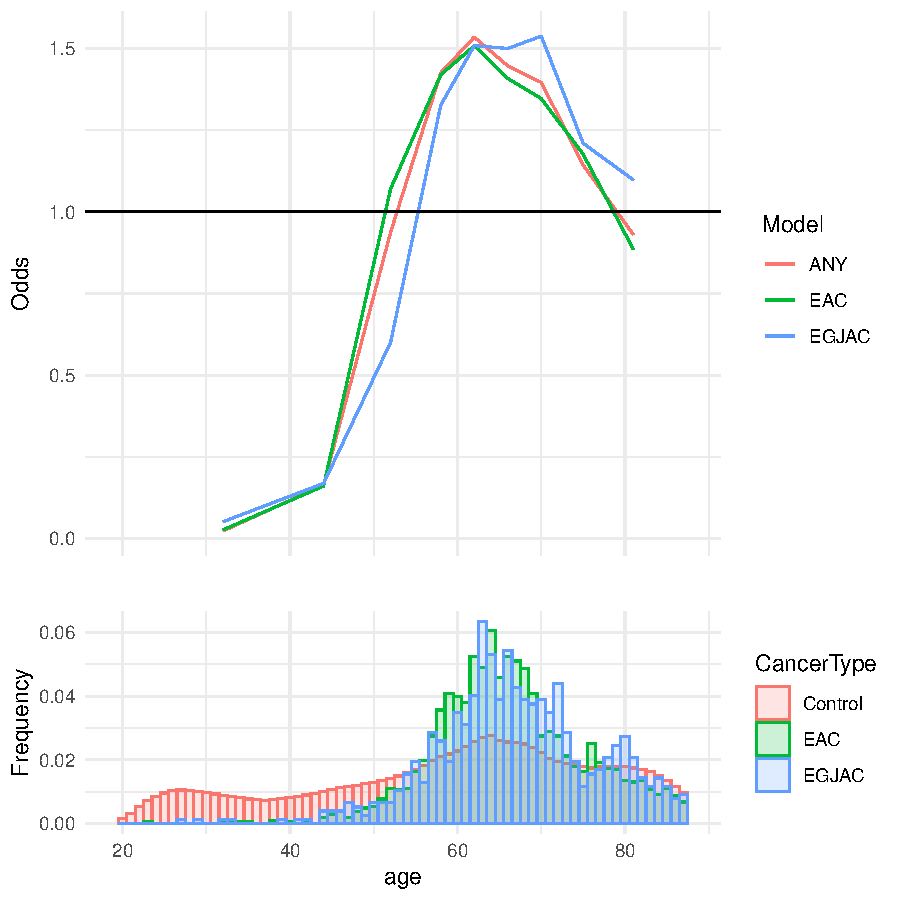
\includegraphics[width=0.45\textwidth]{pdp/age.pdf}
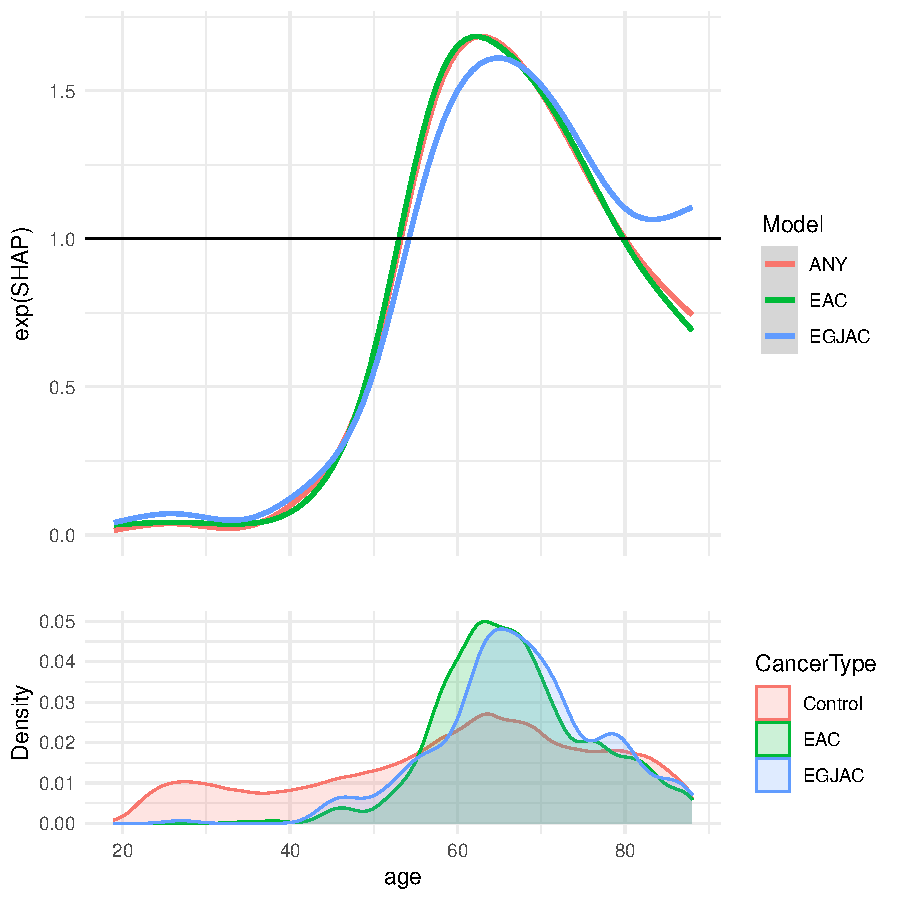
\includegraphics[width=0.45\textwidth]{shap/age.pdf}
\end{figure}
\begin{figure}[h]
\centering
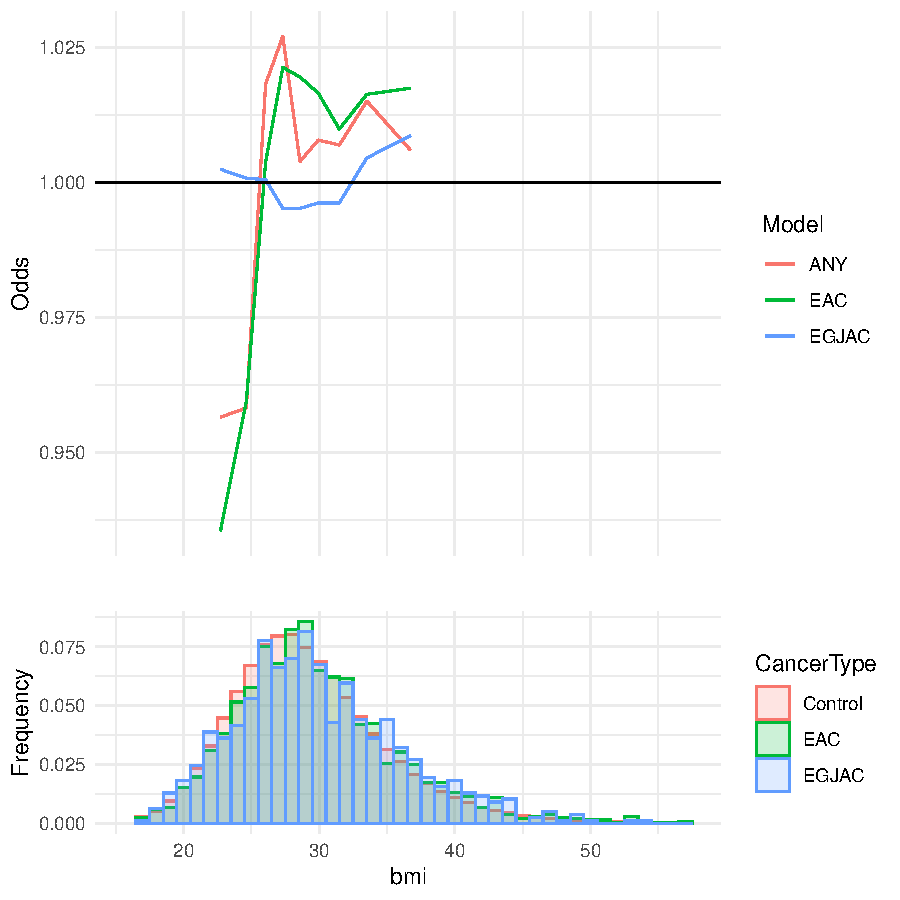
\includegraphics[width=0.45\textwidth]{pdp/bmi.pdf}
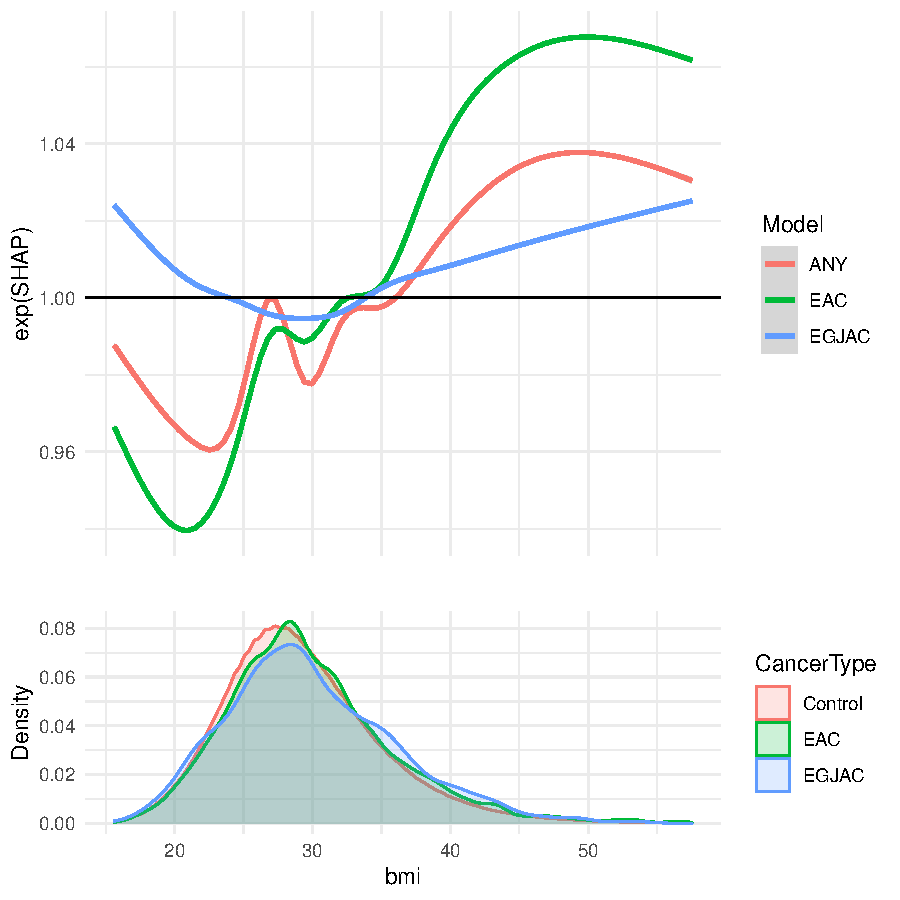
\includegraphics[width=0.45\textwidth]{shap/bmi.pdf}
\end{figure}
\begin{figure}[h]
\centering
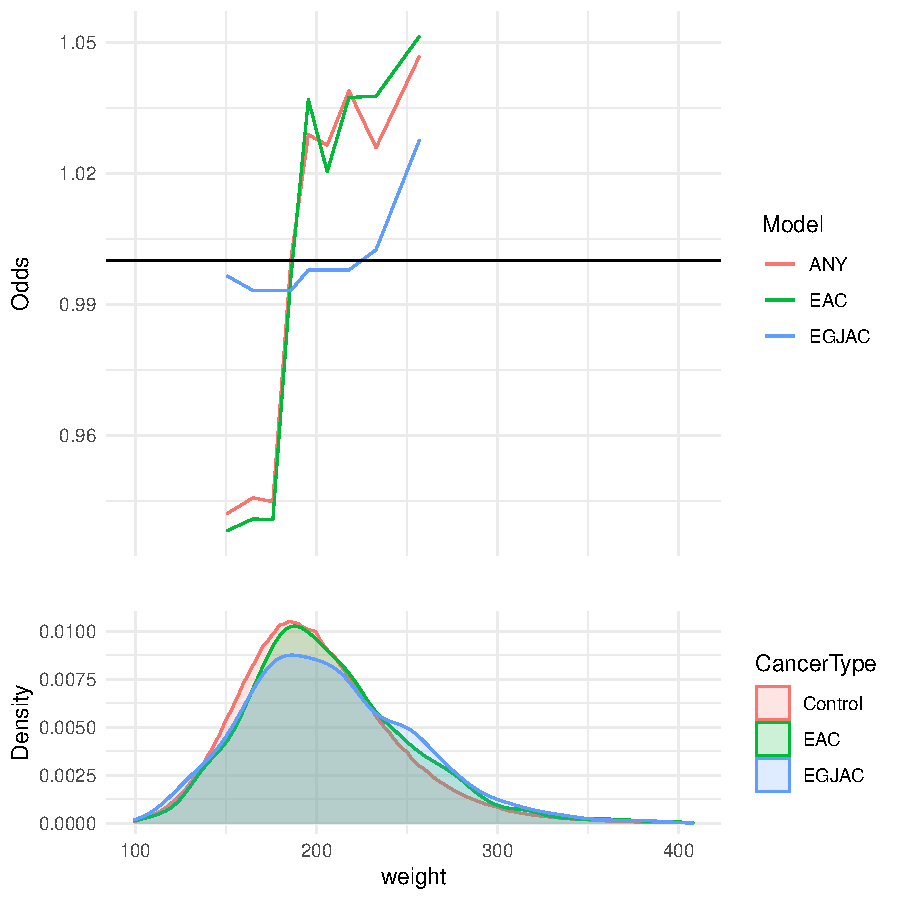
\includegraphics[width=0.45\textwidth]{pdp/weight.pdf}
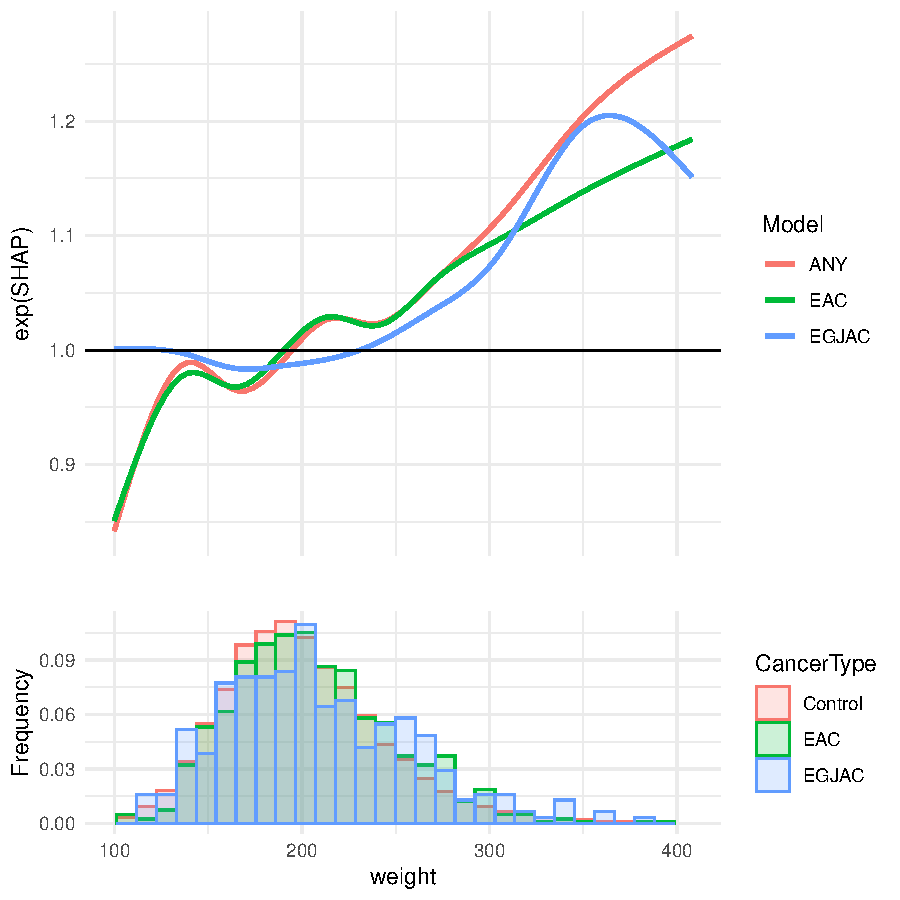
\includegraphics[width=0.45\textwidth]{shap/weight.pdf}
\end{figure}
\begin{figure}[h]
\centering
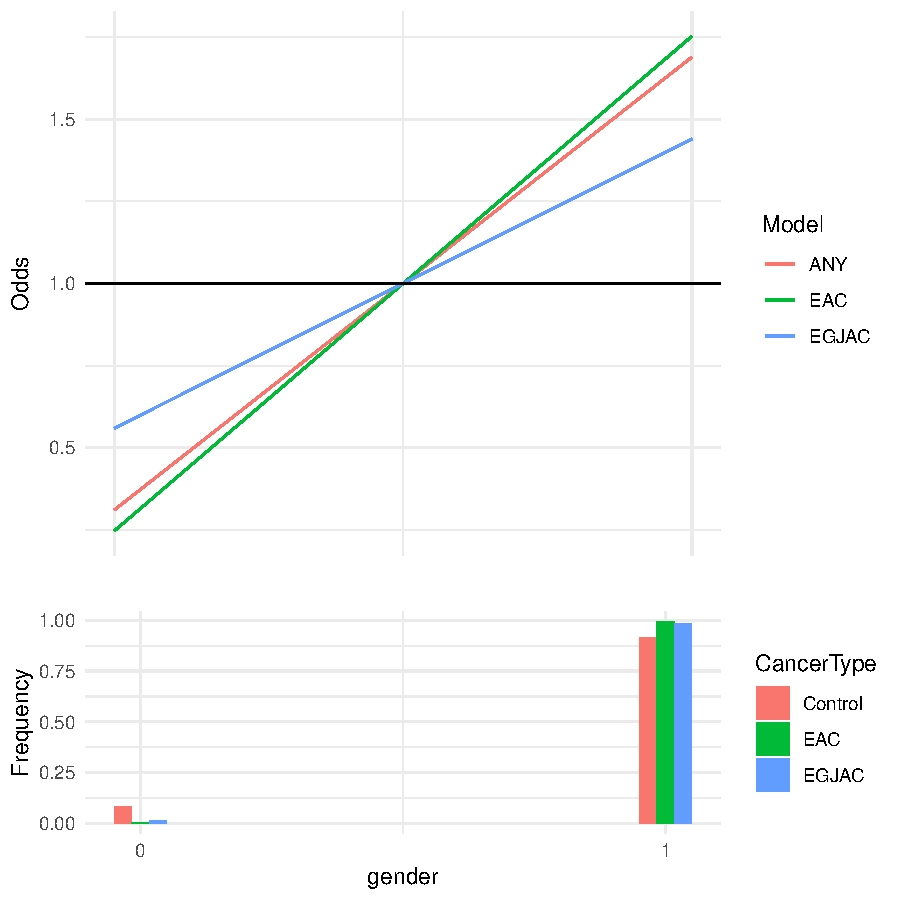
\includegraphics[width=0.45\textwidth]{pdp/gender.pdf}
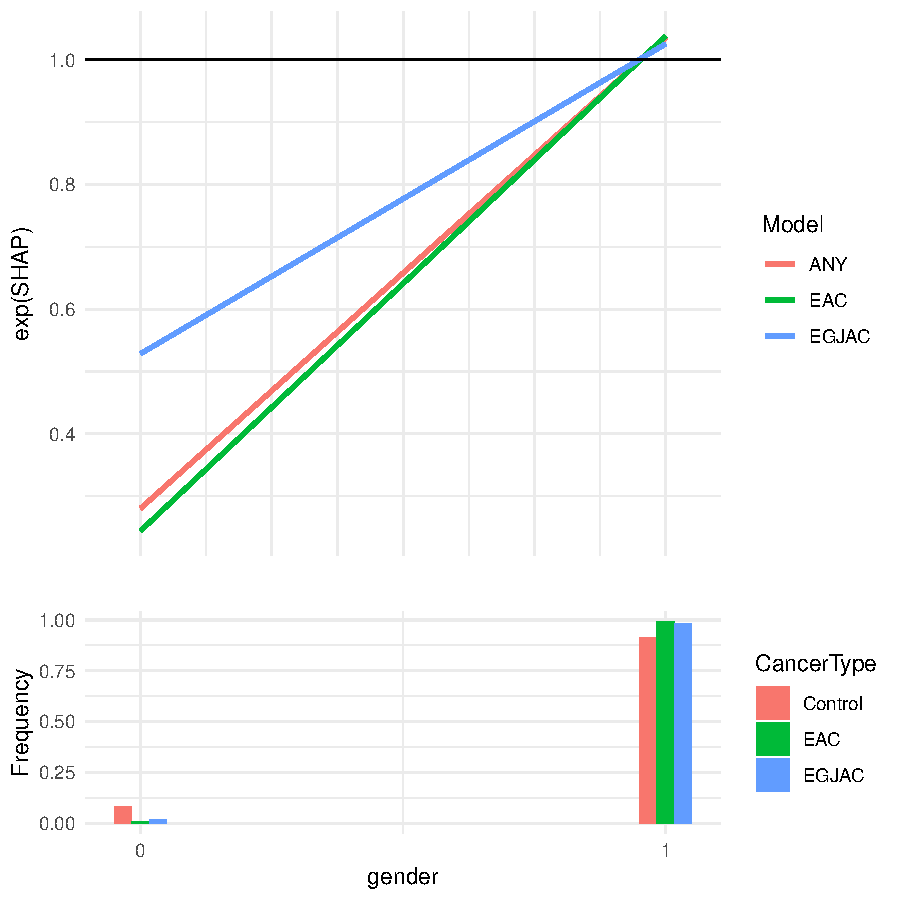
\includegraphics[width=0.45\textwidth]{shap/gender.pdf}
\end{figure}
\begin{figure}[h]
\centering
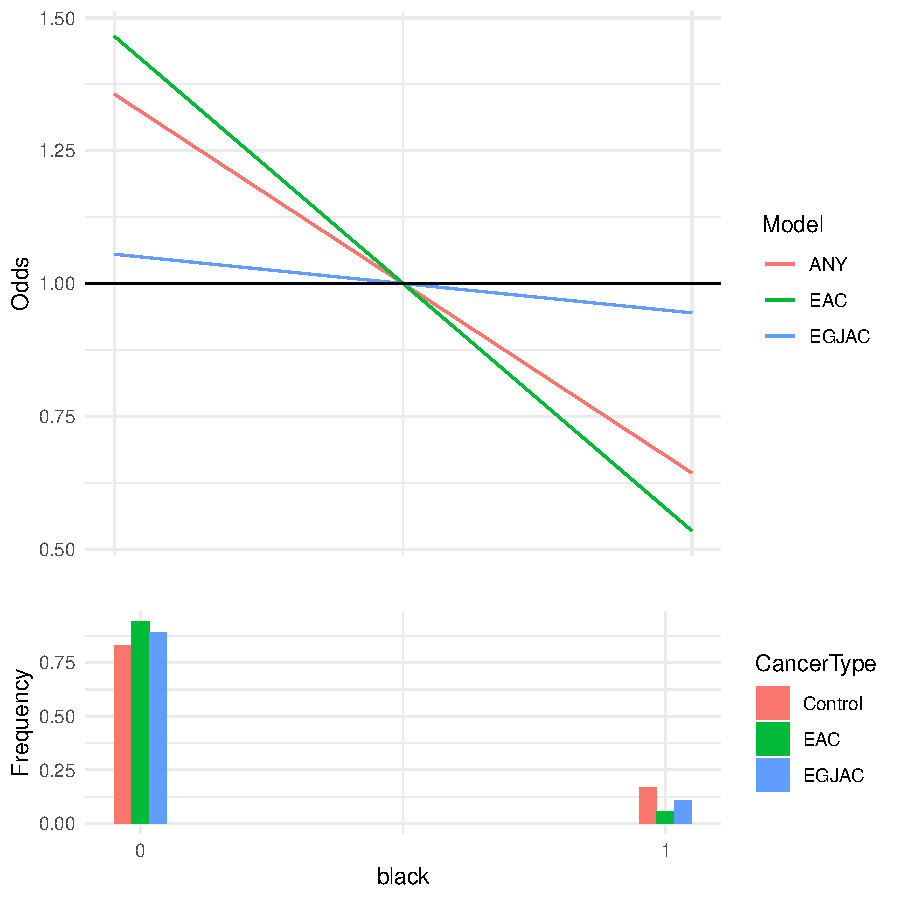
\includegraphics[width=0.45\textwidth]{pdp/black.pdf}
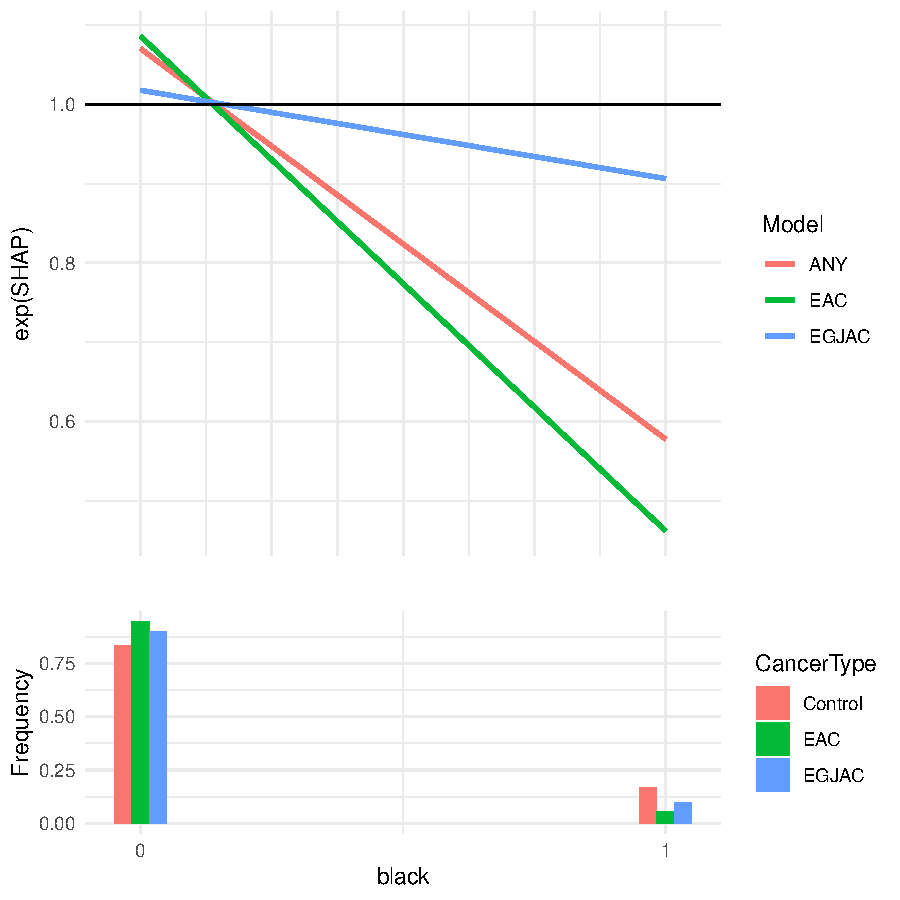
\includegraphics[width=0.45\textwidth]{shap/black.pdf}
\end{figure}
\begin{figure}[h]
\centering
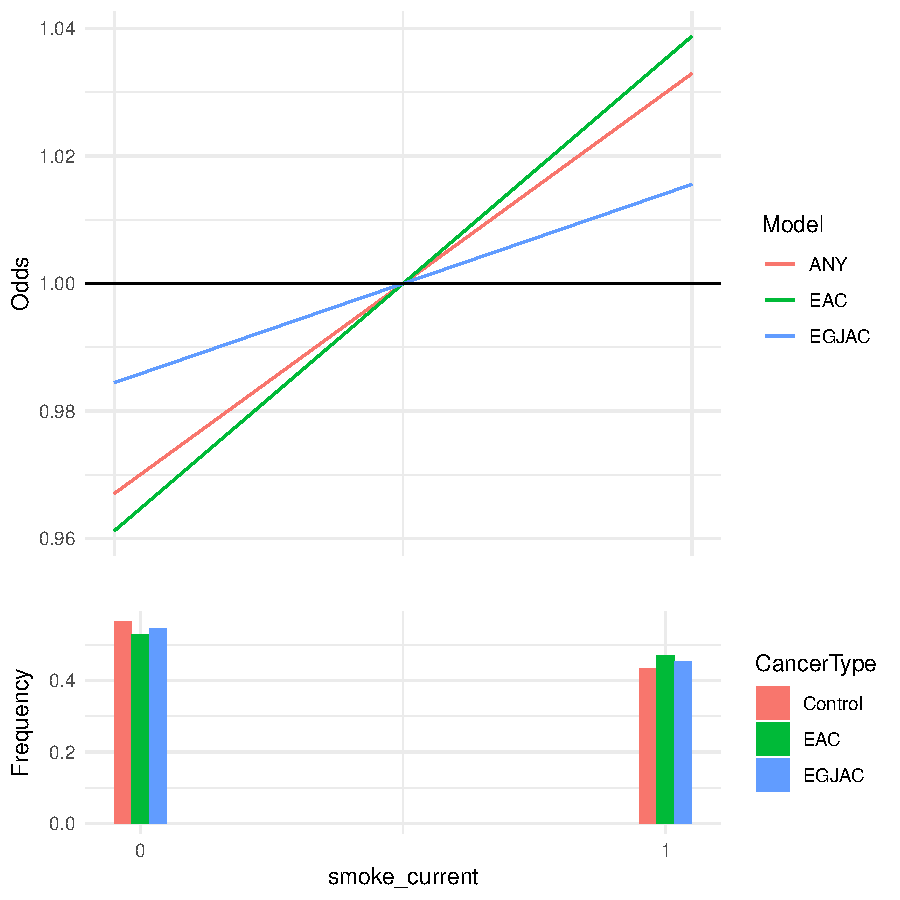
\includegraphics[width=0.45\textwidth]{pdp/smoke_current.pdf}
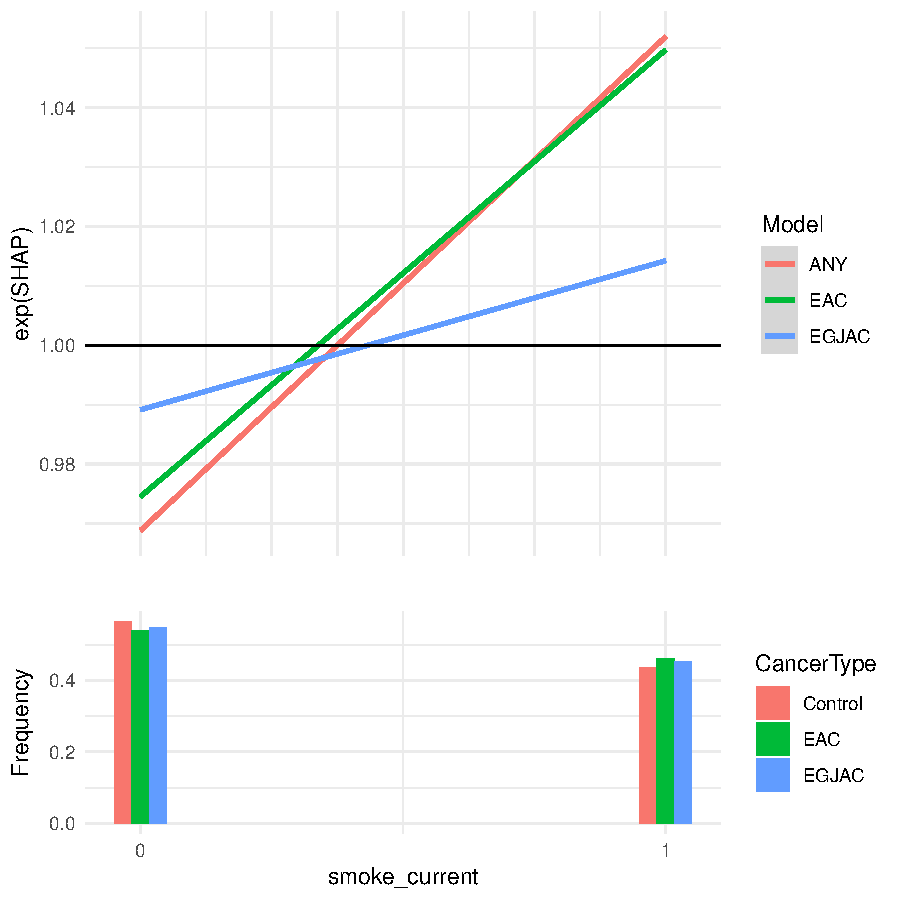
\includegraphics[width=0.45\textwidth]{shap/smoke_current.pdf}
\end{figure}
\begin{figure}[h]
\centering
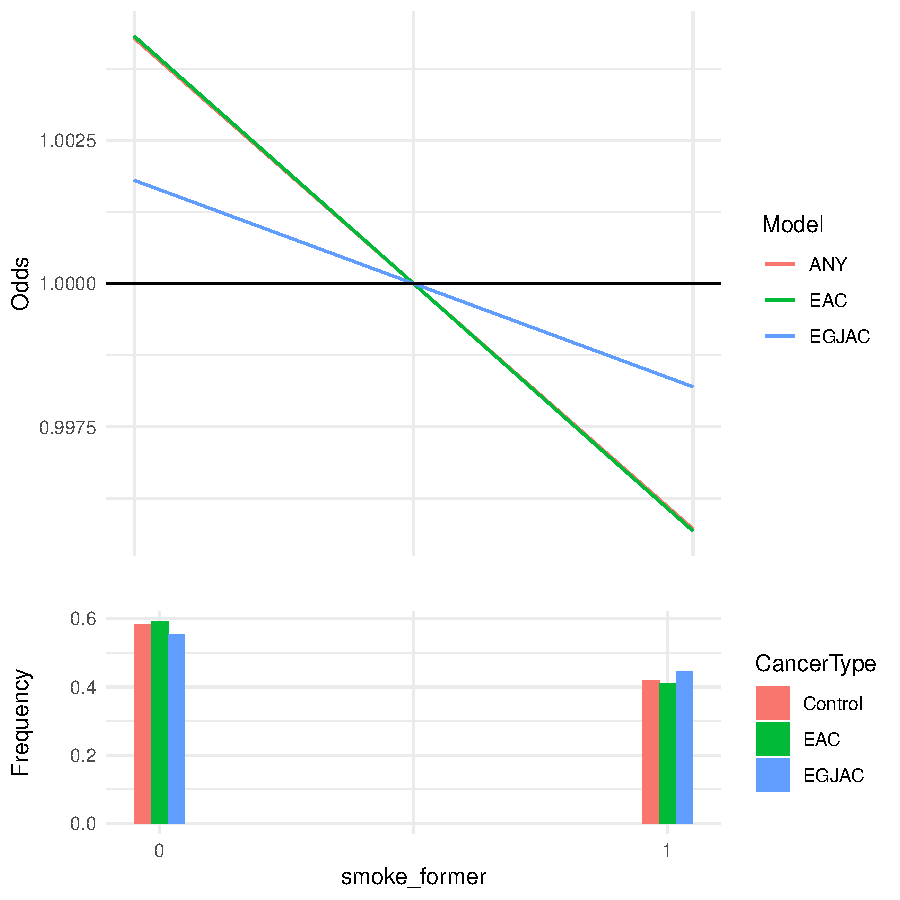
\includegraphics[width=0.45\textwidth]{pdp/smoke_former.pdf}
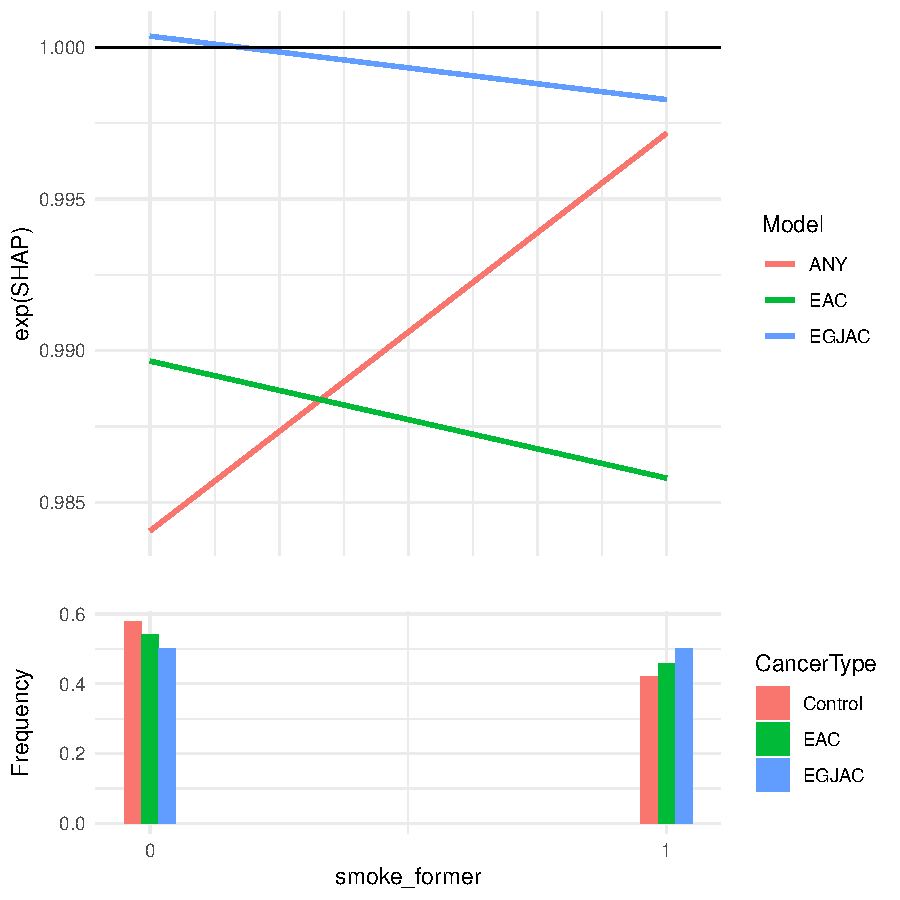
\includegraphics[width=0.45\textwidth]{shap/smoke_former.pdf}
\end{figure}



\newpage
\clearpage
\section{Comorbidities}

\begin{figure}[h]
\centering
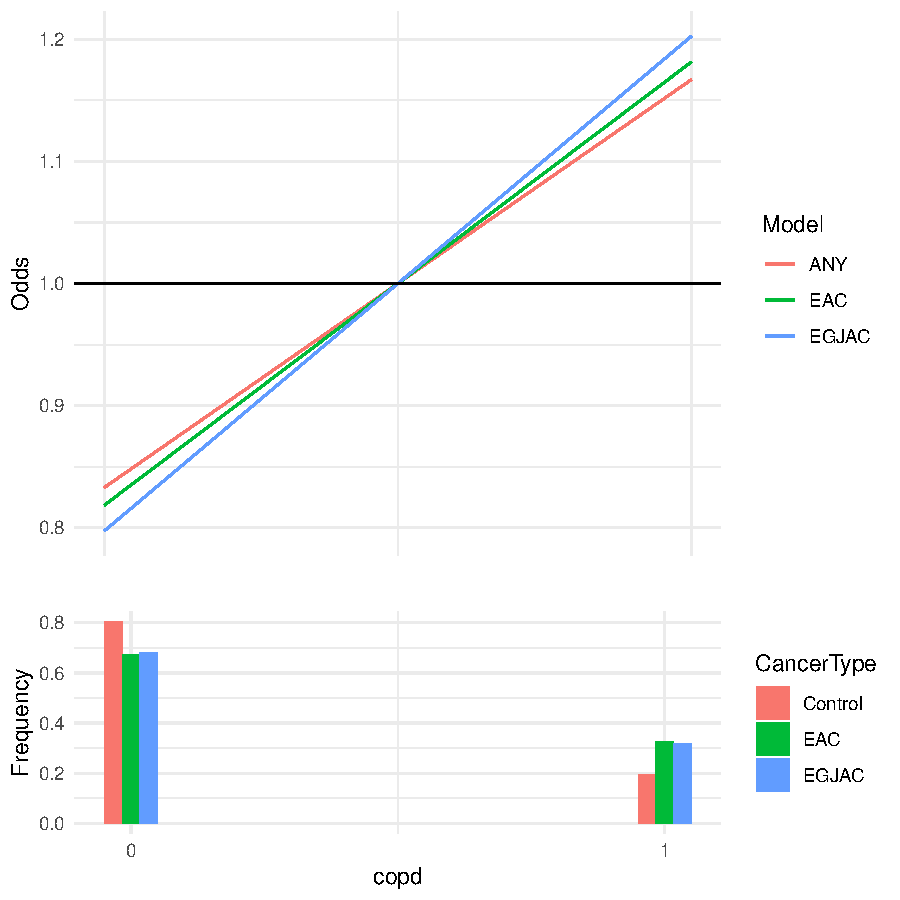
\includegraphics[width=0.45\textwidth]{pdp/copd.pdf}
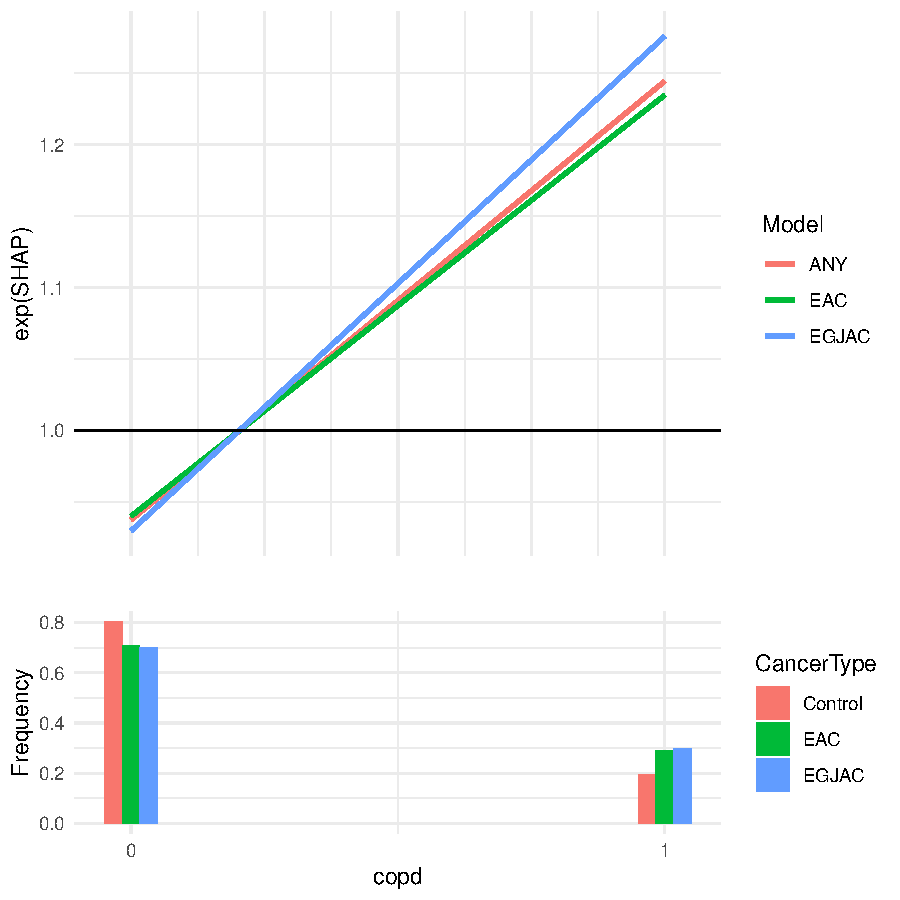
\includegraphics[width=0.45\textwidth]{shap/copd.pdf}
\end{figure}
\begin{figure}[h]
\centering
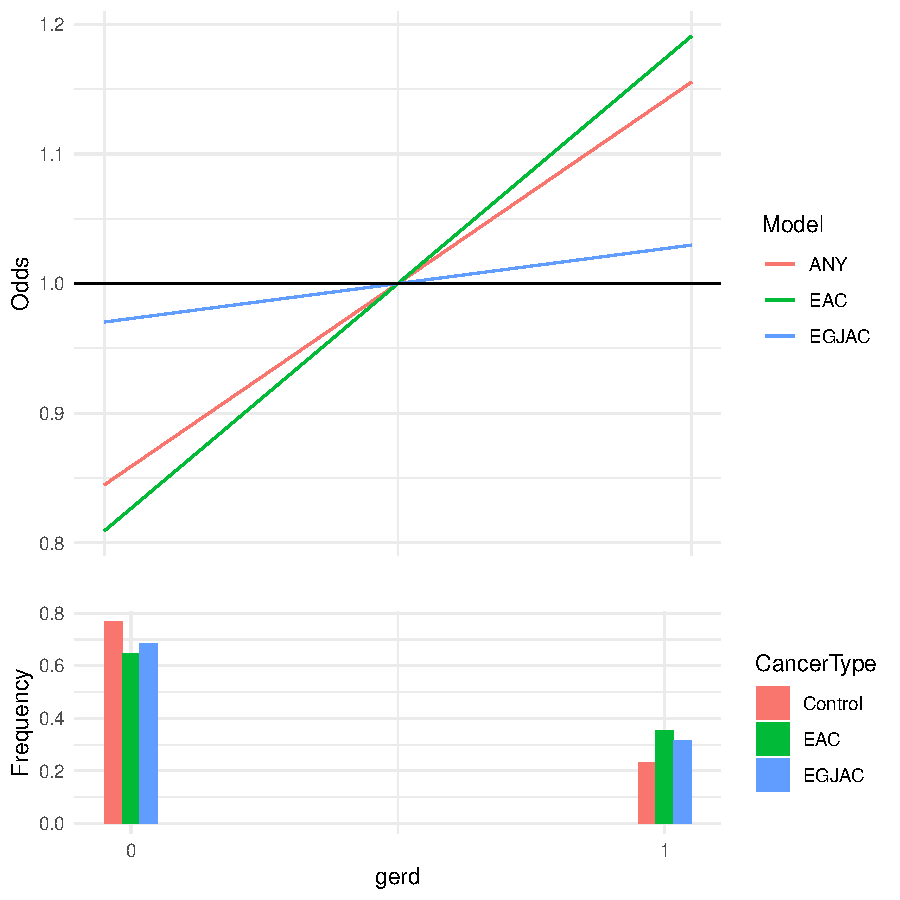
\includegraphics[width=0.45\textwidth]{pdp/gerd.pdf}
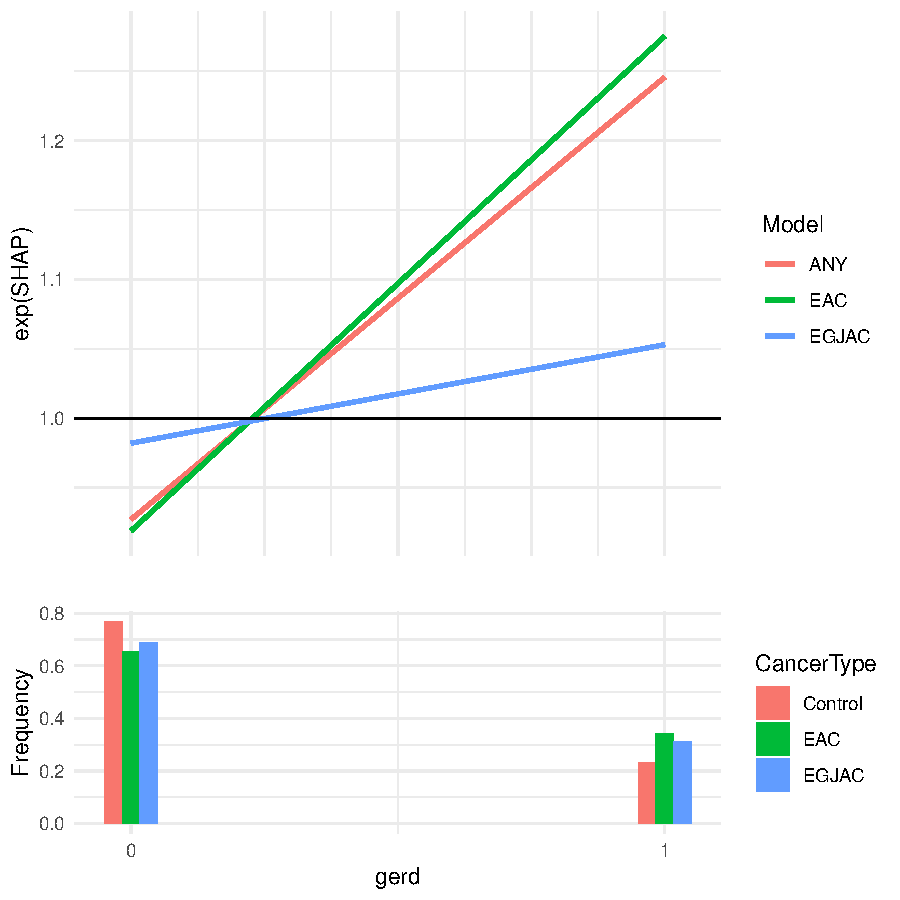
\includegraphics[width=0.45\textwidth]{shap/gerd.pdf}
\end{figure}

\newpage
\clearpage
\section{WBC}

\begin{figure}[h]
\centering
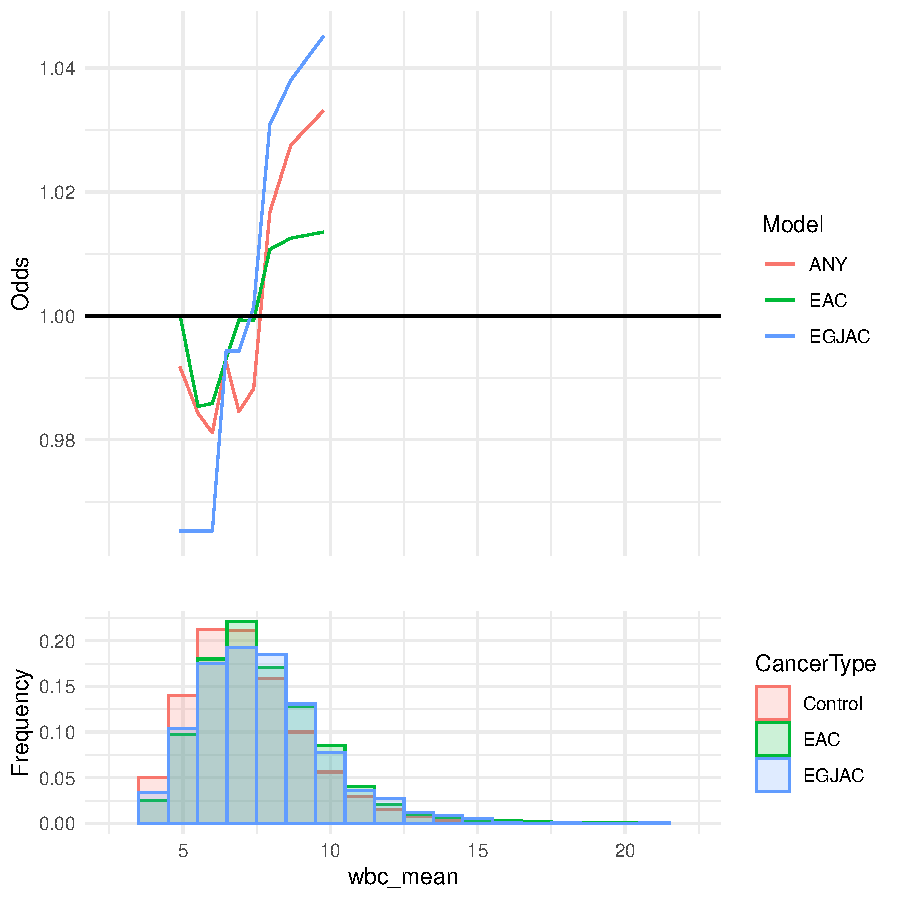
\includegraphics[width=0.45\textwidth]{pdp/wbc_mean.pdf}
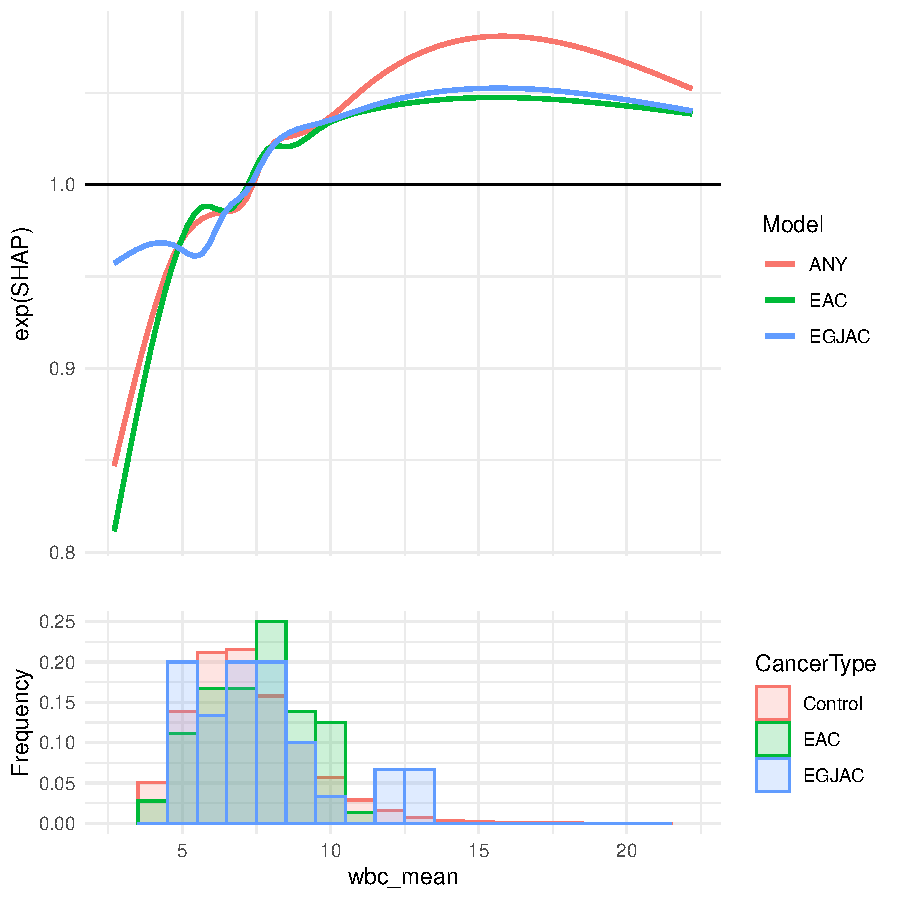
\includegraphics[width=0.45\textwidth]{shap/wbc_mean.pdf}
\end{figure}
\begin{figure}[h]
\centering
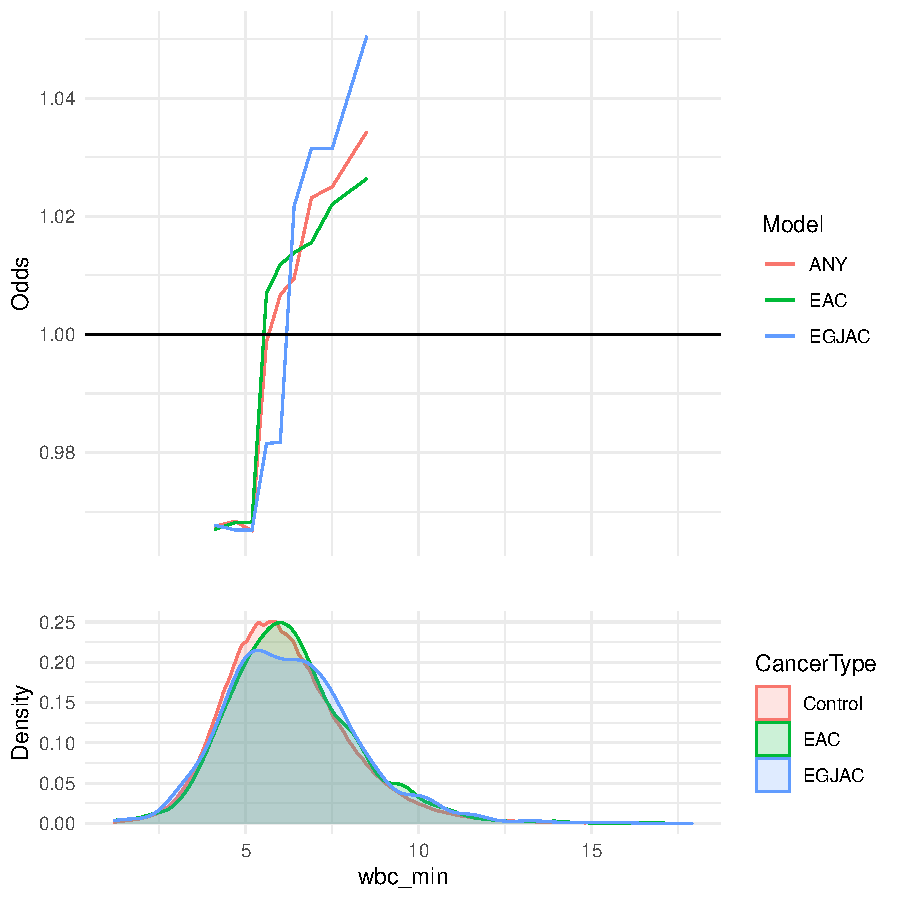
\includegraphics[width=0.45\textwidth]{pdp/wbc_min.pdf}
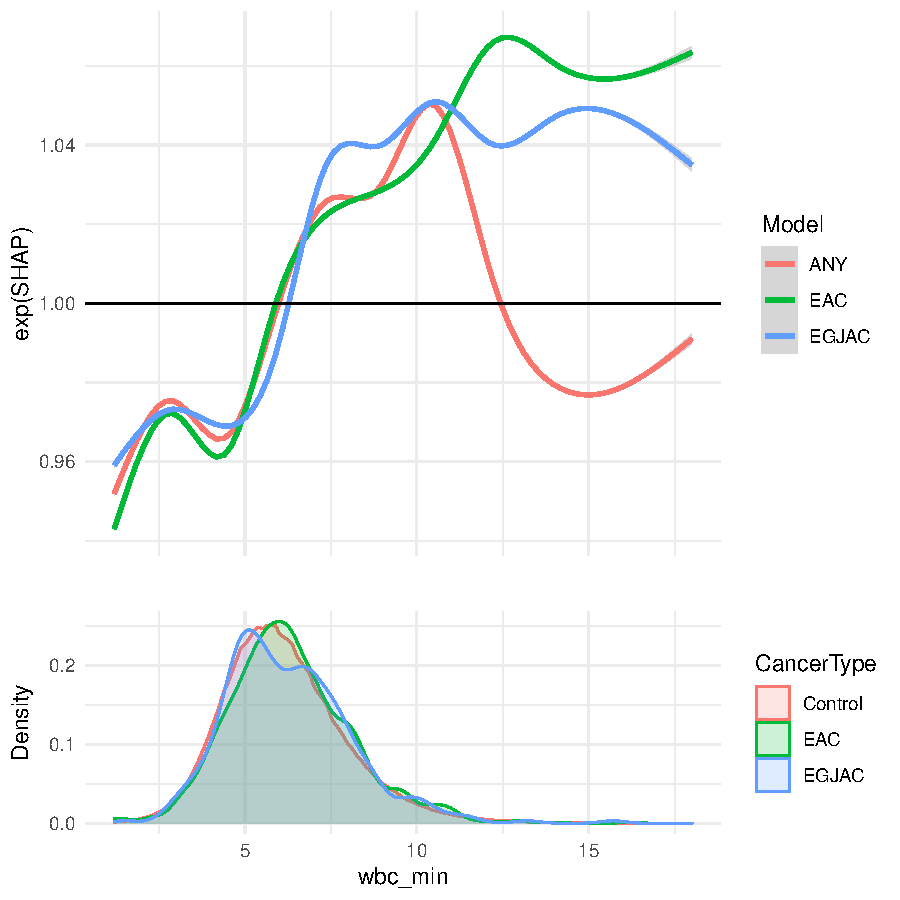
\includegraphics[width=0.45\textwidth]{shap/wbc_min.pdf}
\end{figure}
\begin{figure}[h]
\centering
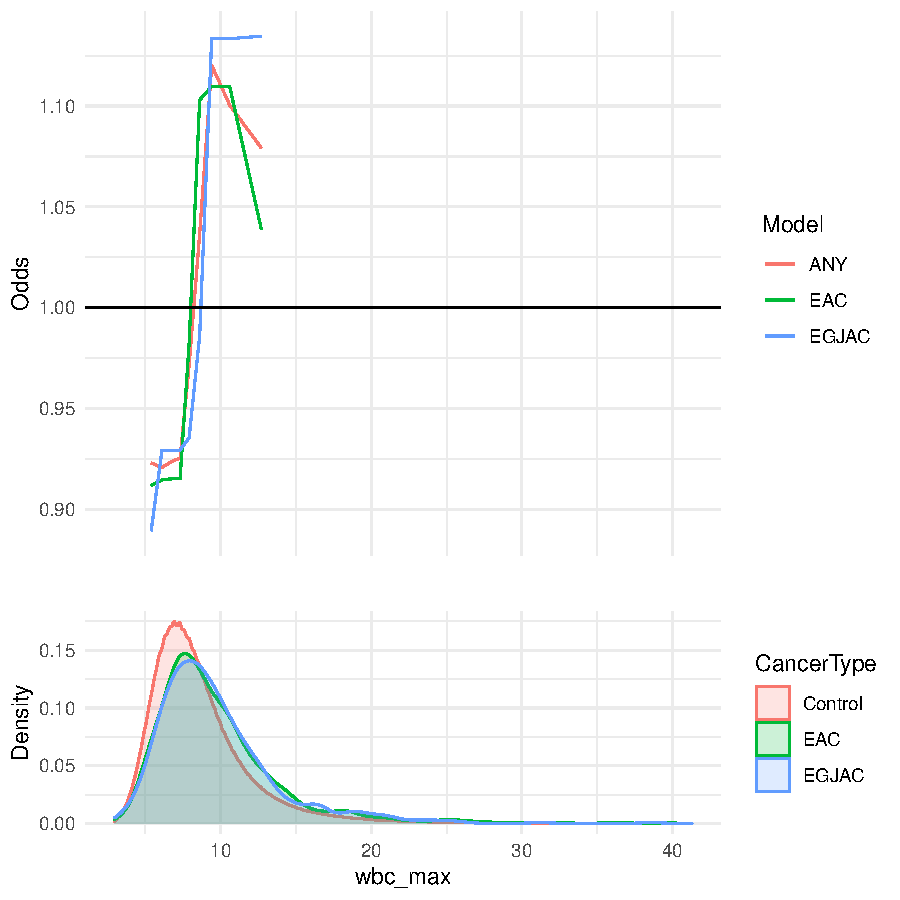
\includegraphics[width=0.45\textwidth]{pdp/wbc_max.pdf}
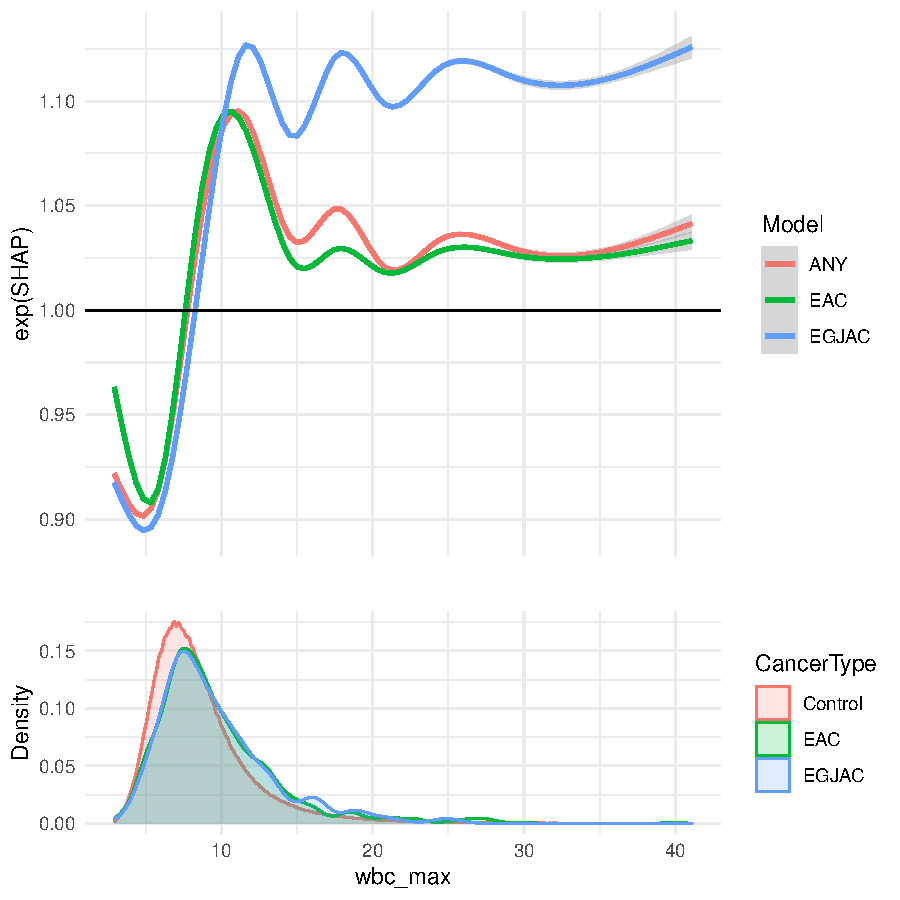
\includegraphics[width=0.45\textwidth]{shap/wbc_max.pdf}
\end{figure}
\begin{figure}[h]
\centering
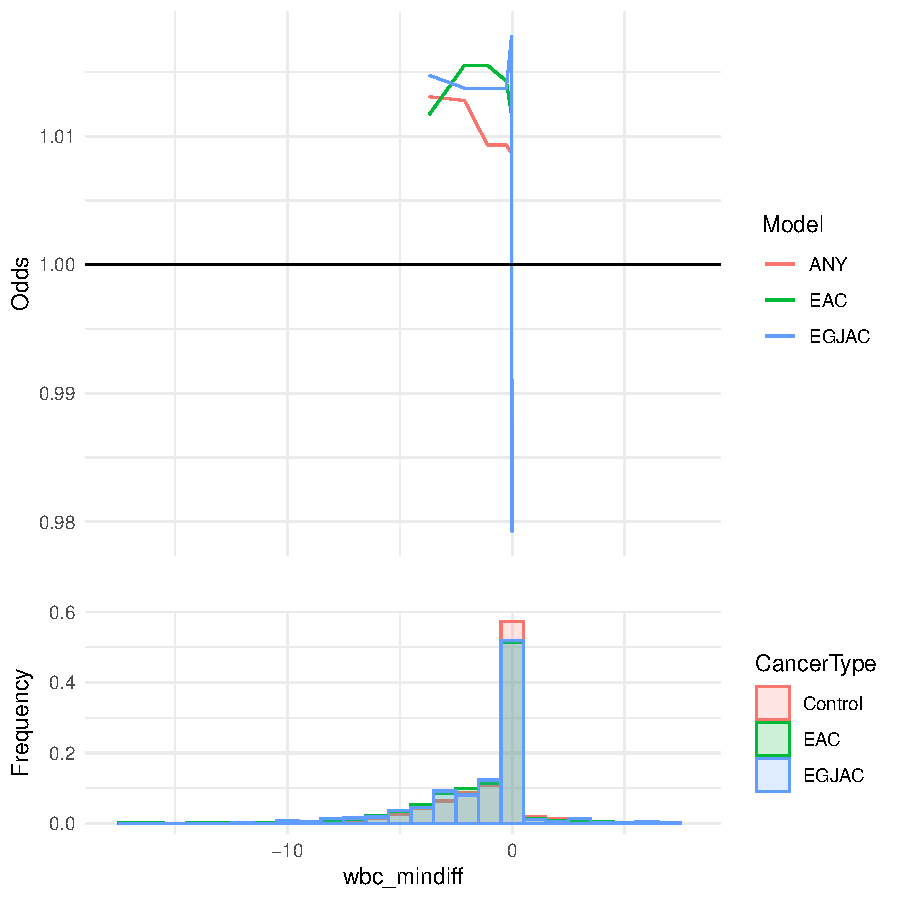
\includegraphics[width=0.45\textwidth]{pdp/wbc_mindiff.pdf}
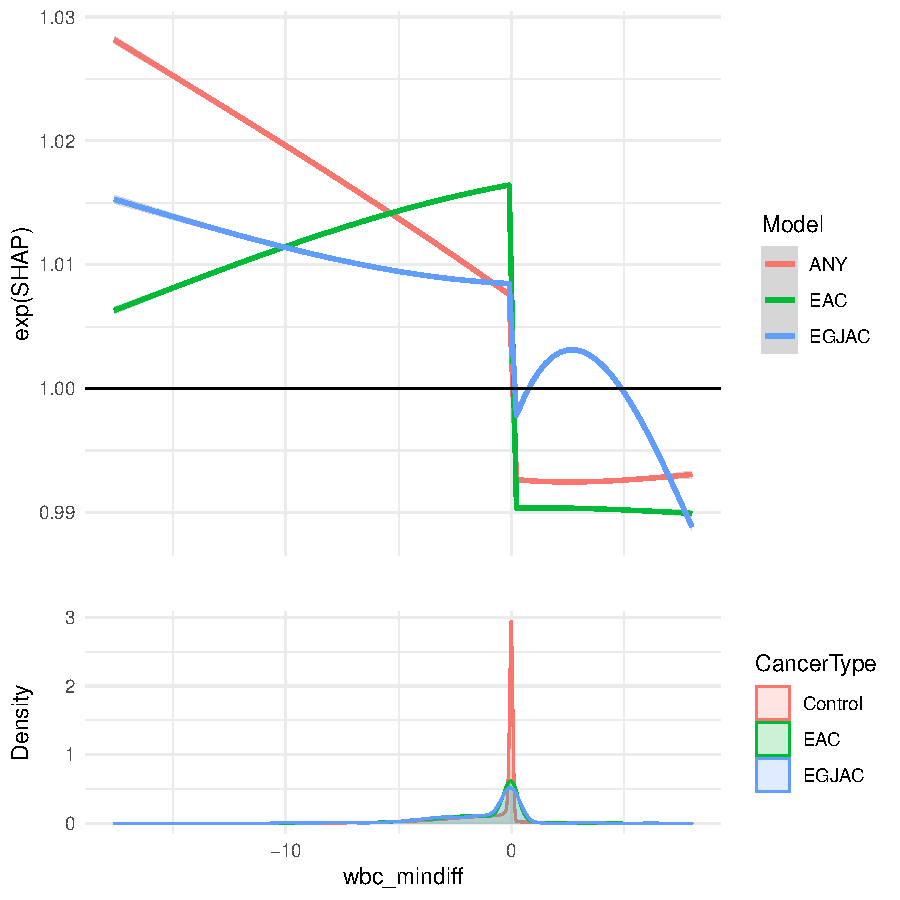
\includegraphics[width=0.45\textwidth]{shap/wbc_mindiff.pdf}
\end{figure}
\begin{figure}[h]
\centering
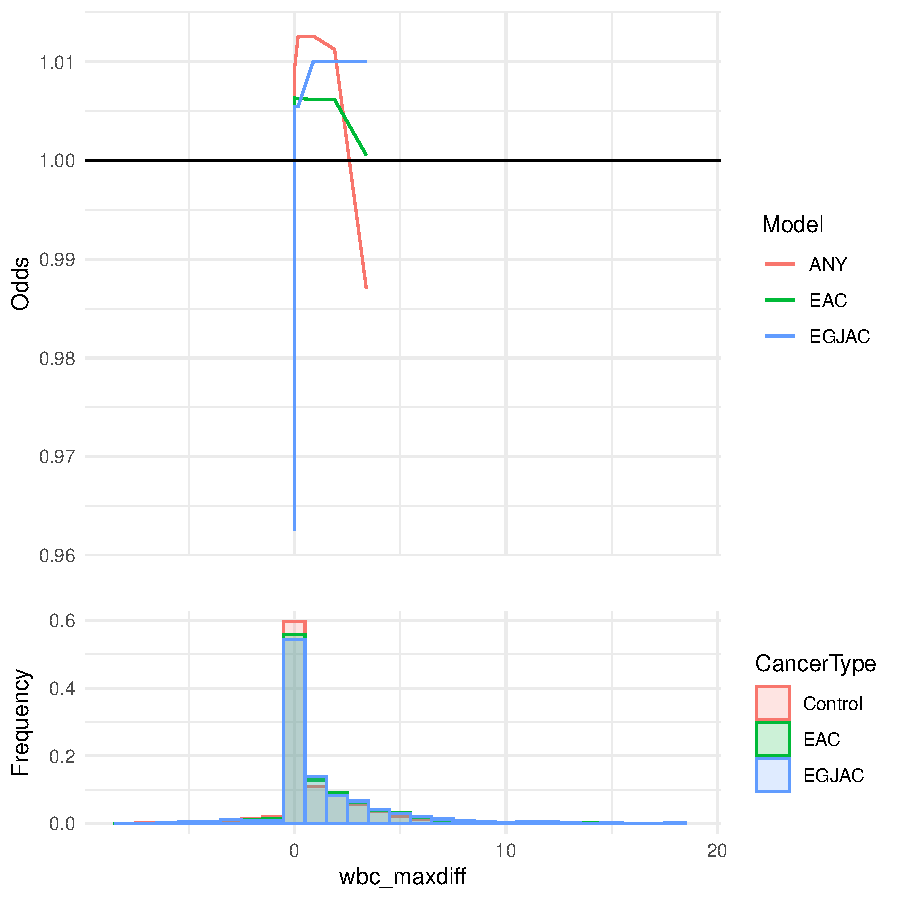
\includegraphics[width=0.45\textwidth]{pdp/wbc_maxdiff.pdf}
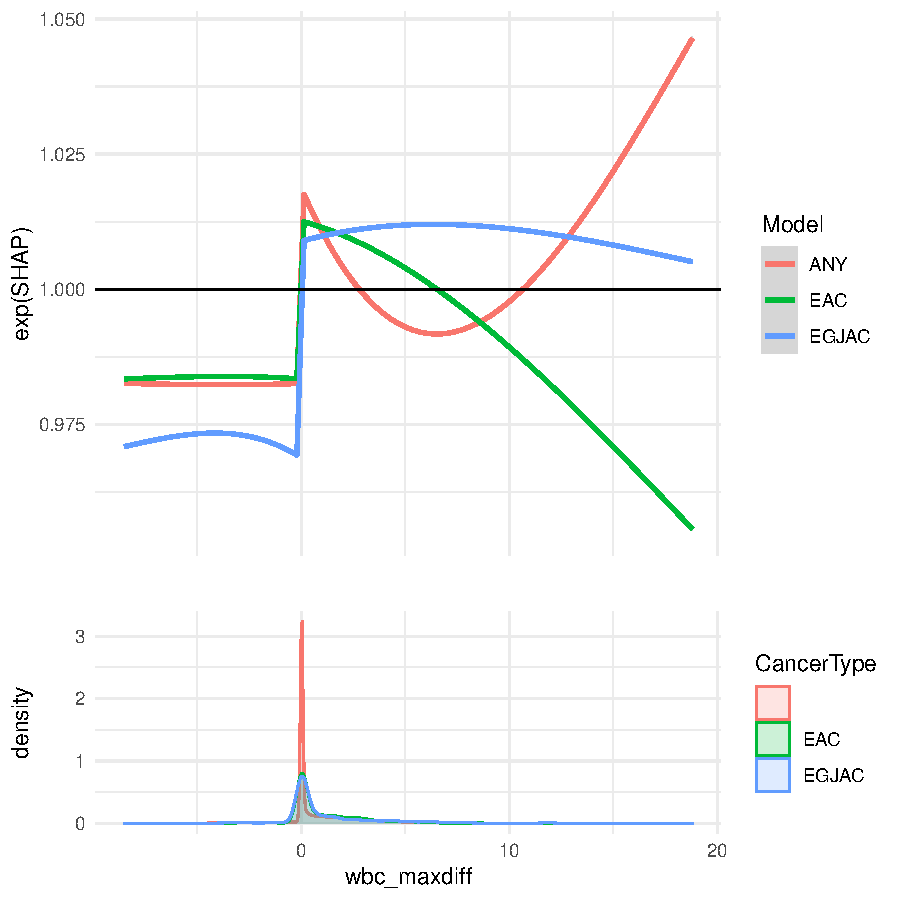
\includegraphics[width=0.45\textwidth]{shap/wbc_maxdiff.pdf}
\end{figure}
\begin{figure}[h]
\centering
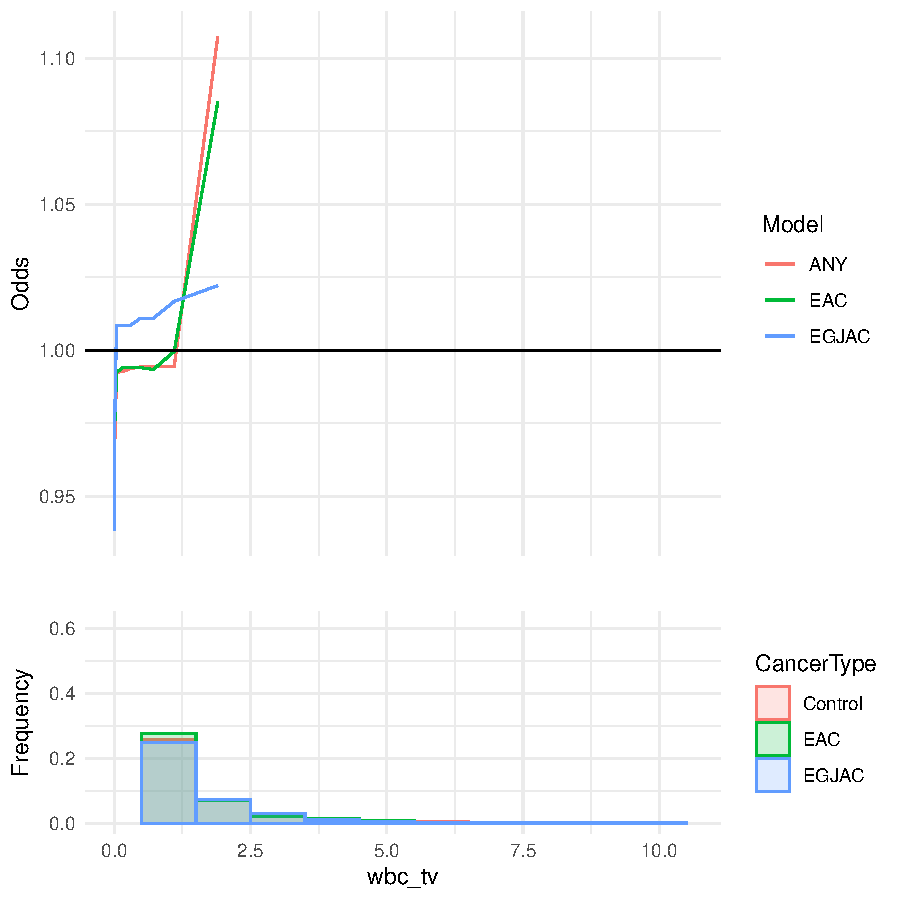
\includegraphics[width=0.45\textwidth]{pdp/wbc_tv.pdf}
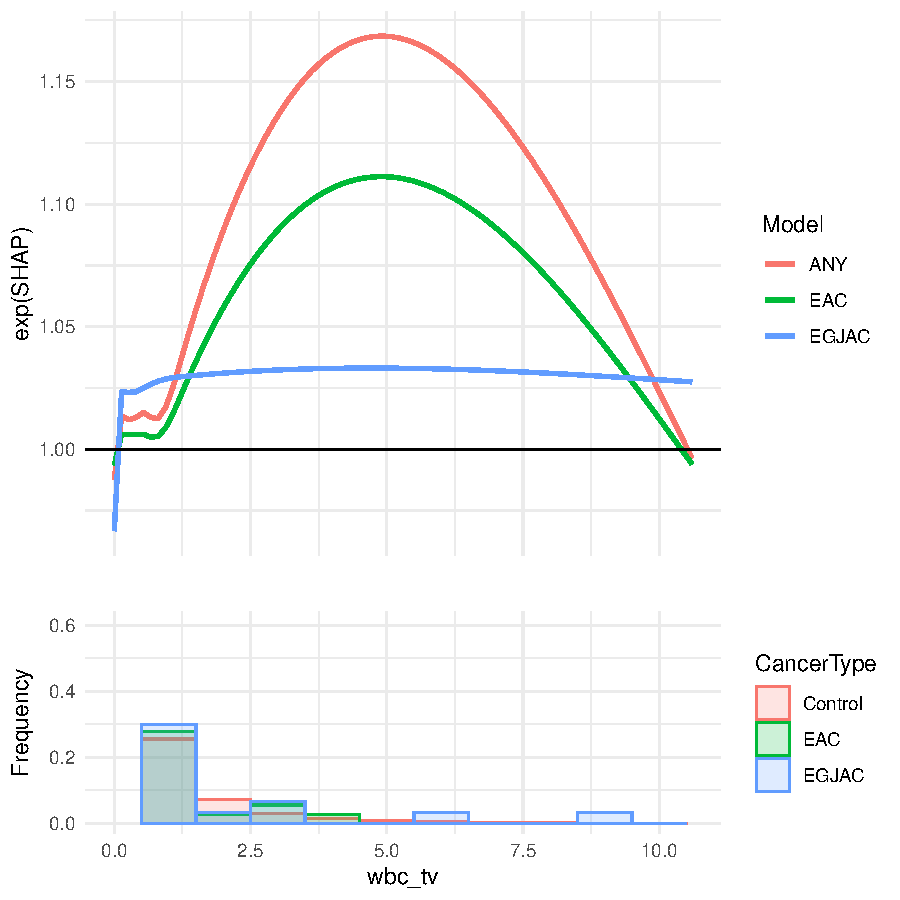
\includegraphics[width=0.45\textwidth]{shap/wbc_tv.pdf}
\end{figure}



\newpage
\clearpage
\section{NA}

\begin{figure}[h]
\centering
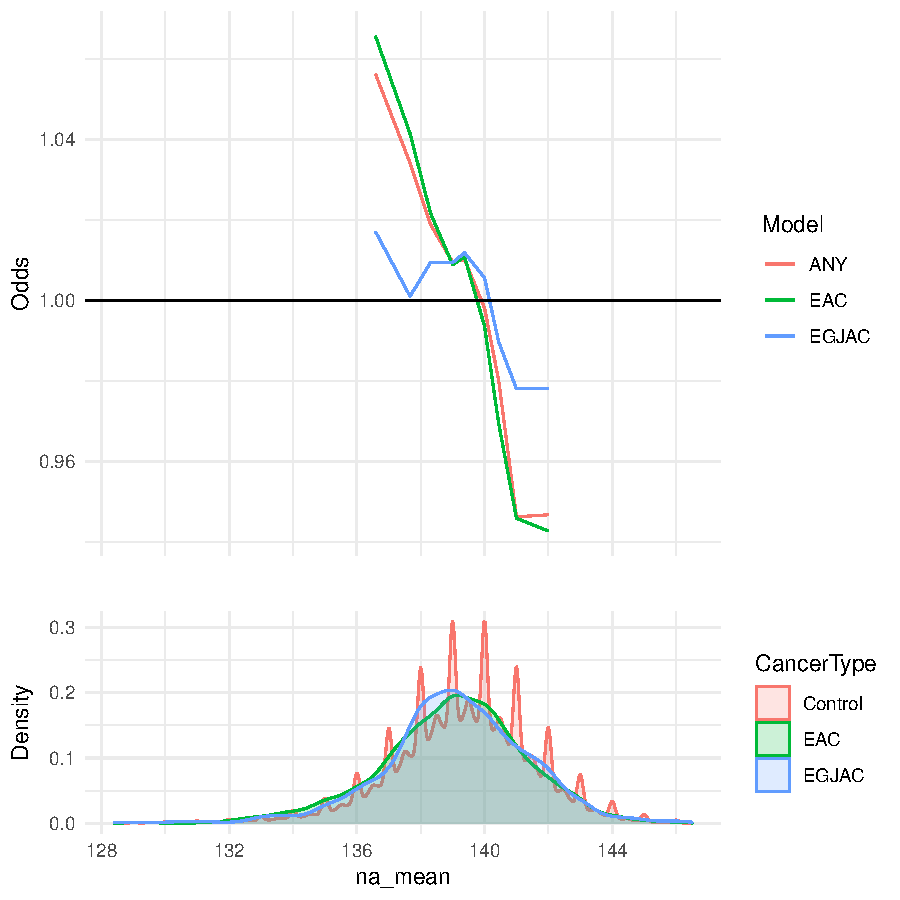
\includegraphics[width=0.45\textwidth]{pdp/na_mean.pdf}
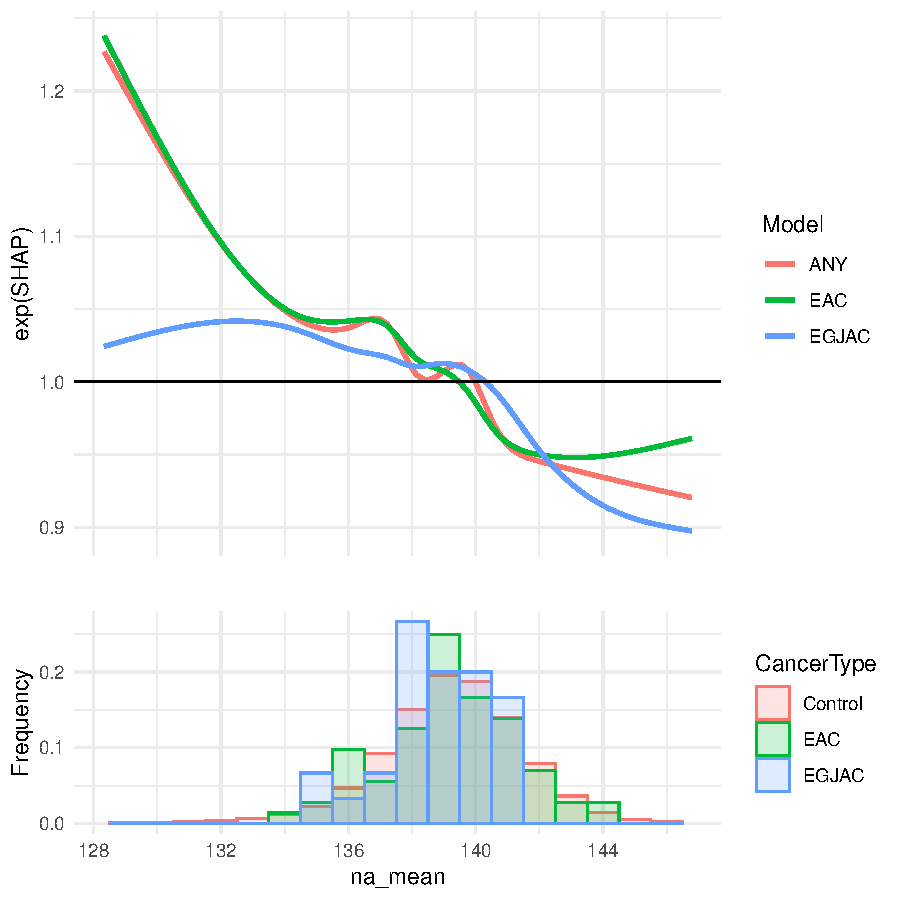
\includegraphics[width=0.45\textwidth]{shap/na_mean.pdf}
\end{figure}
\begin{figure}[h]
\centering
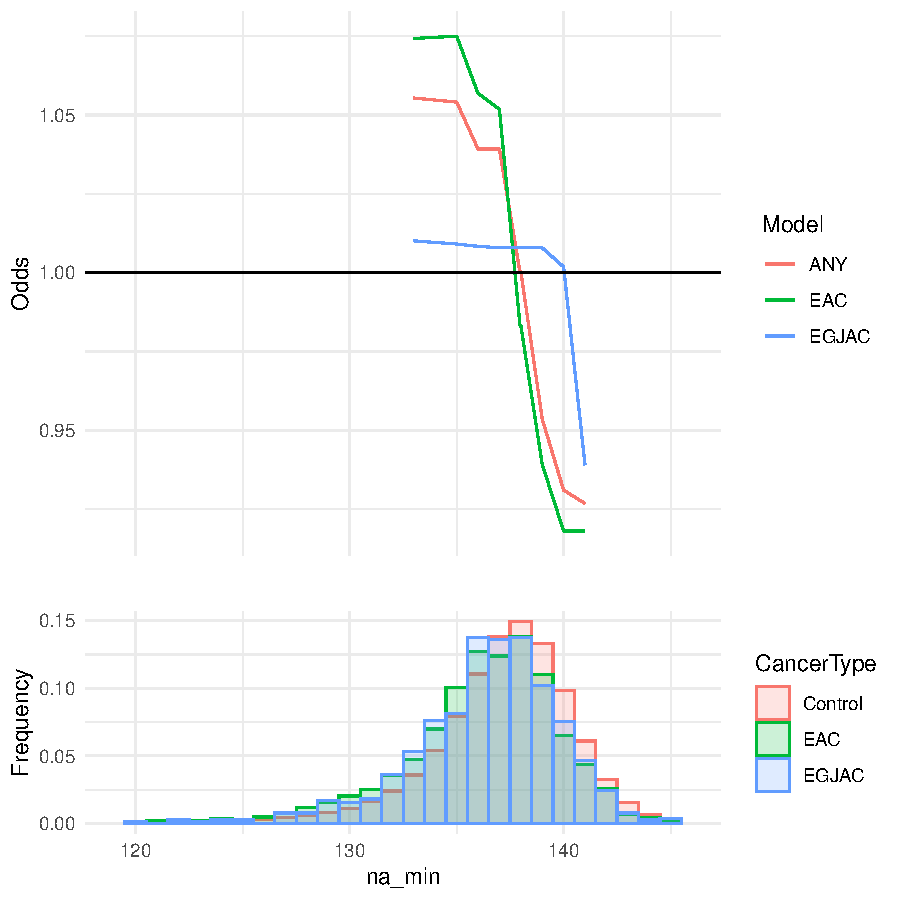
\includegraphics[width=0.45\textwidth]{pdp/na_min.pdf}
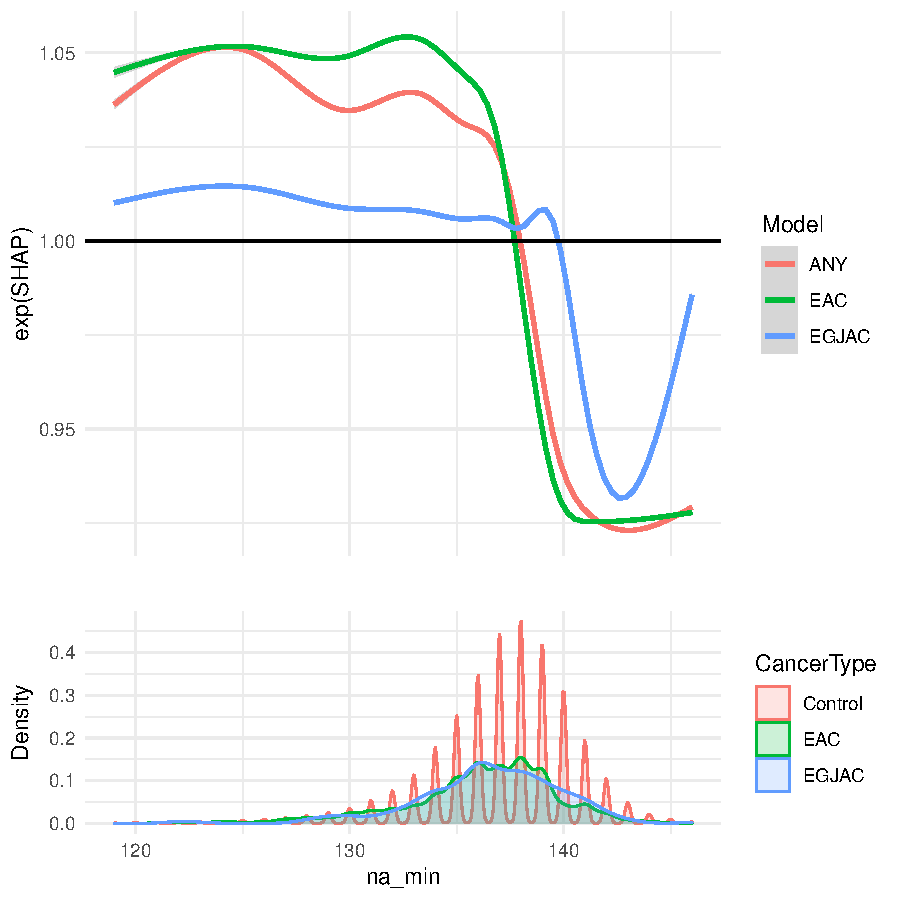
\includegraphics[width=0.45\textwidth]{shap/na_min.pdf}
\end{figure}
\begin{figure}[h]
\centering
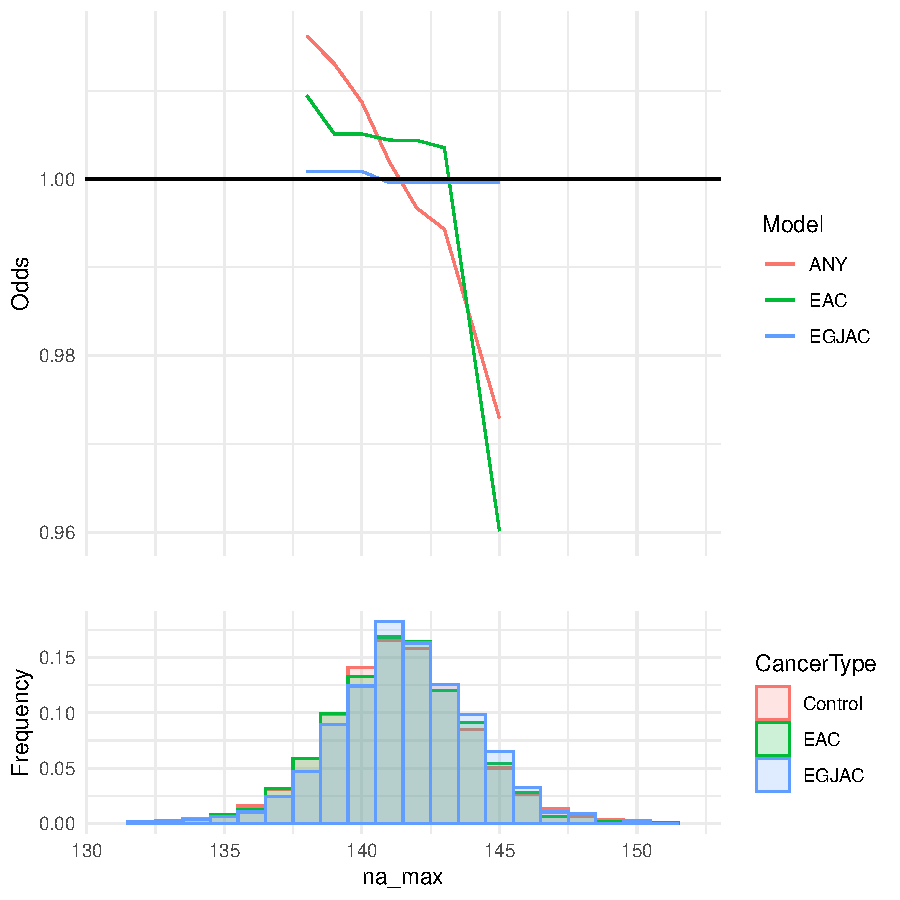
\includegraphics[width=0.45\textwidth]{pdp/na_max.pdf}
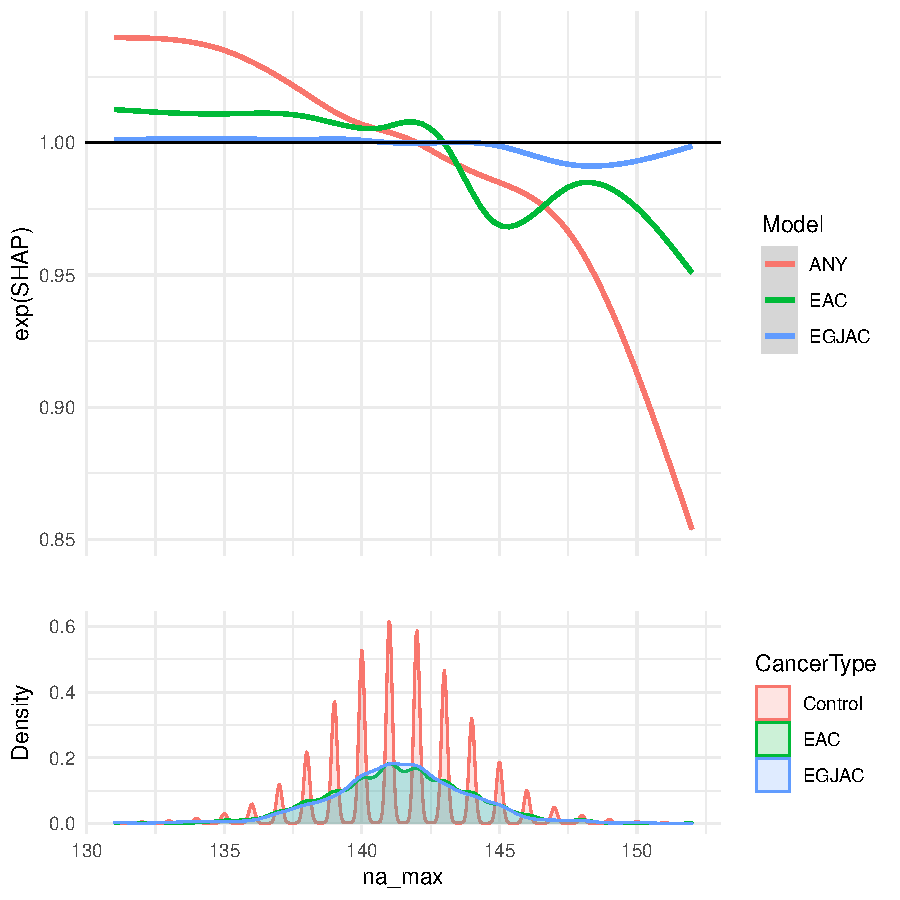
\includegraphics[width=0.45\textwidth]{shap/na_max.pdf}
\end{figure}
\begin{figure}[h]
\centering
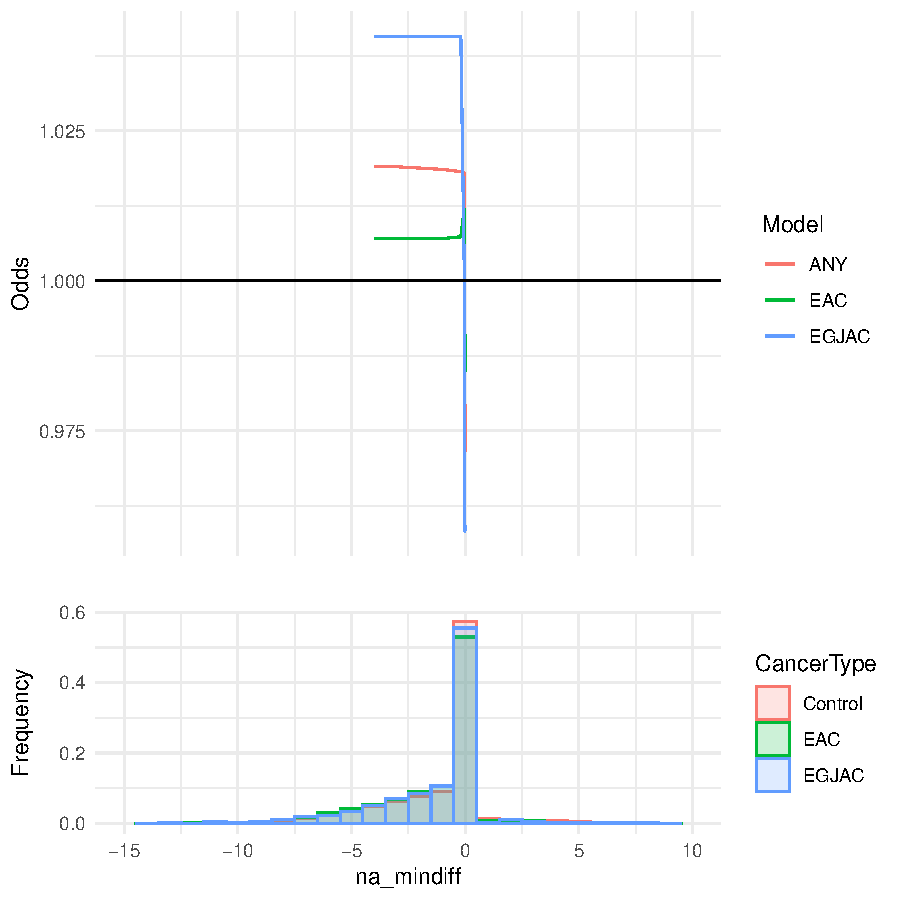
\includegraphics[width=0.45\textwidth]{pdp/na_mindiff.pdf}
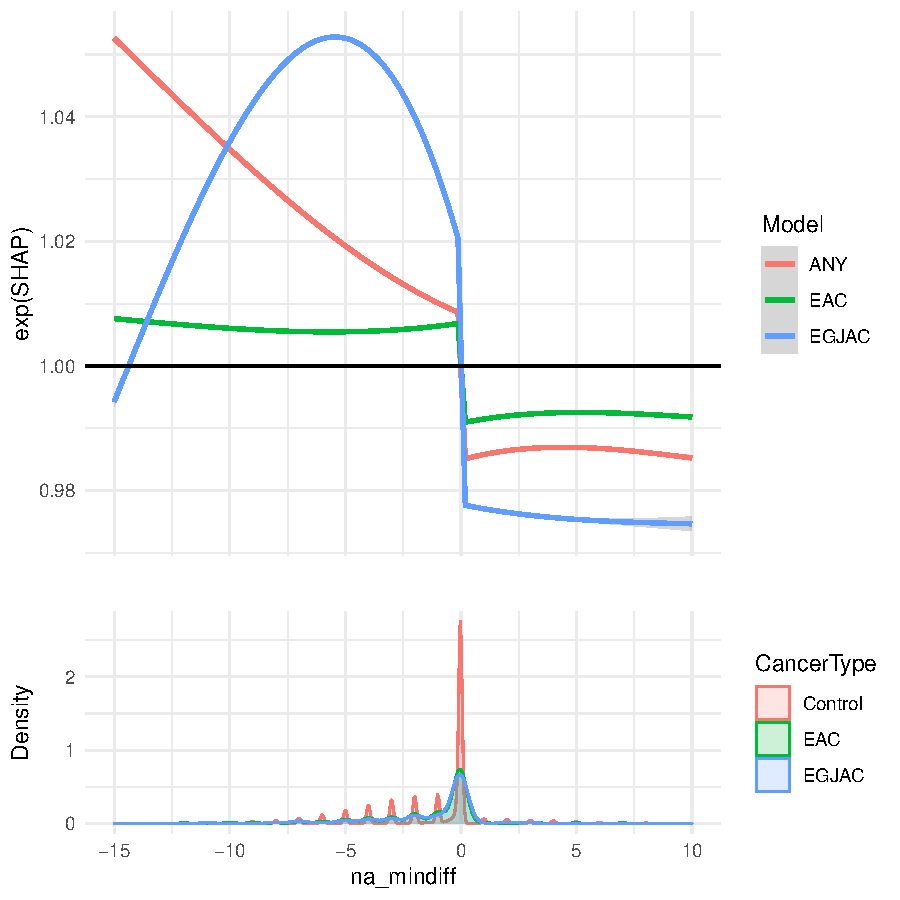
\includegraphics[width=0.45\textwidth]{shap/na_mindiff.pdf}
\end{figure}
\begin{figure}[h]
\centering
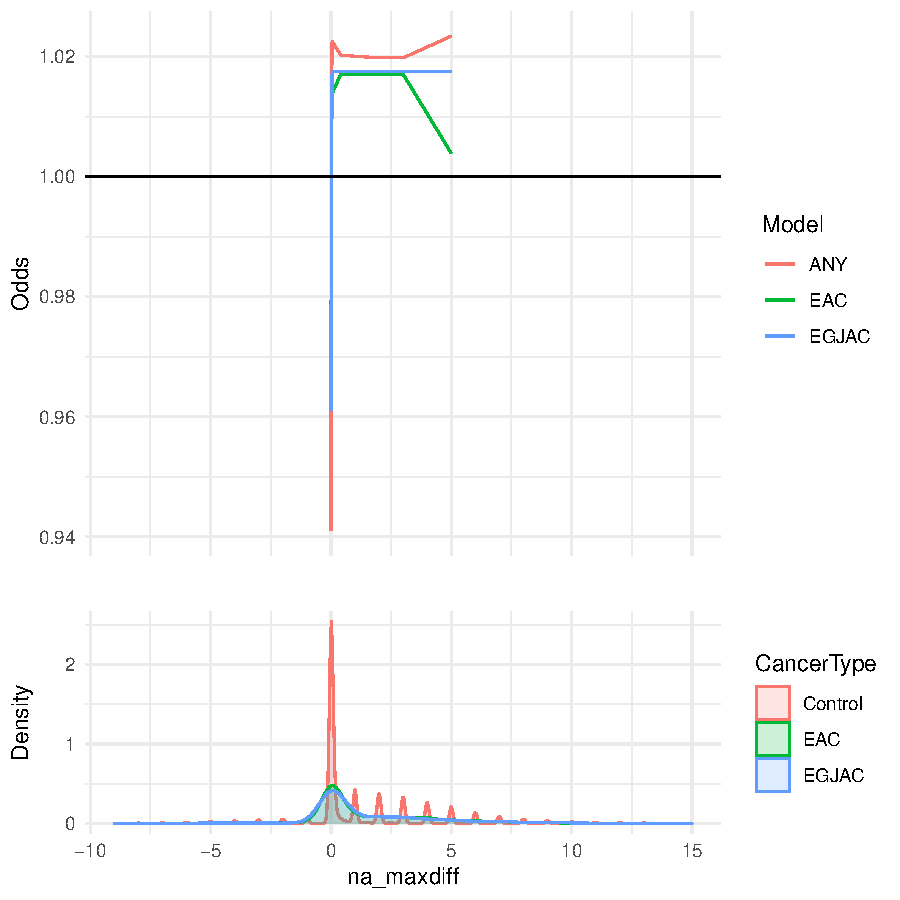
\includegraphics[width=0.45\textwidth]{pdp/na_maxdiff.pdf}
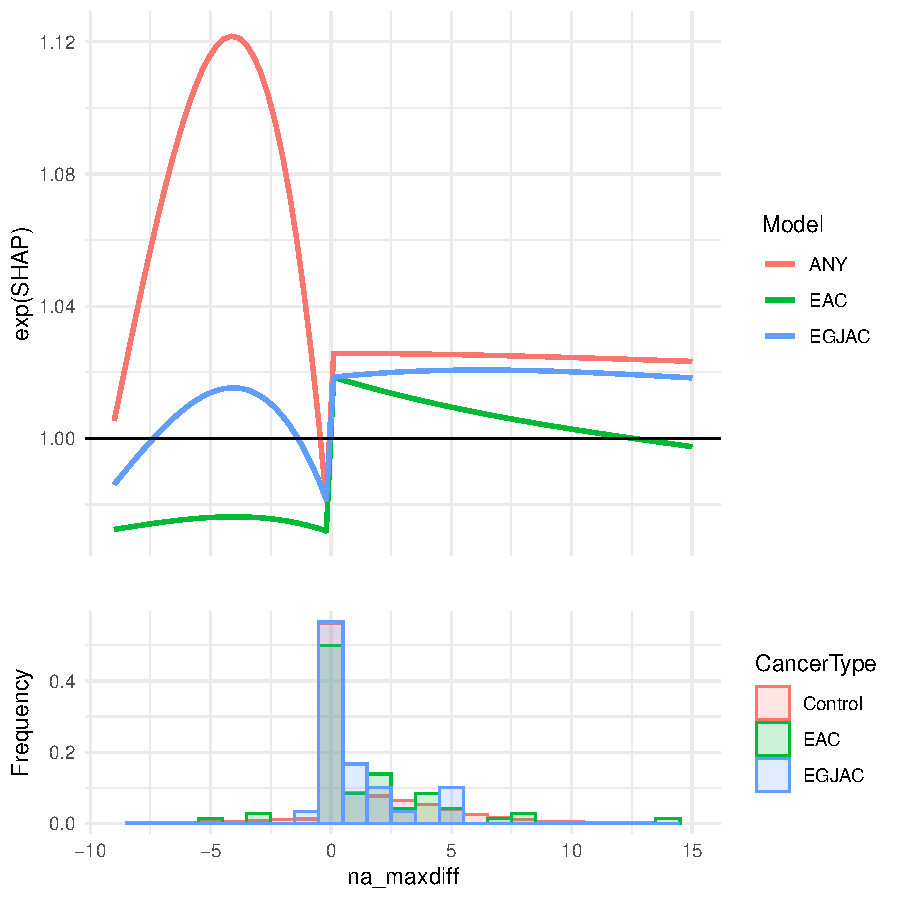
\includegraphics[width=0.45\textwidth]{shap/na_maxdiff.pdf}
\end{figure}
\begin{figure}[h]
\centering
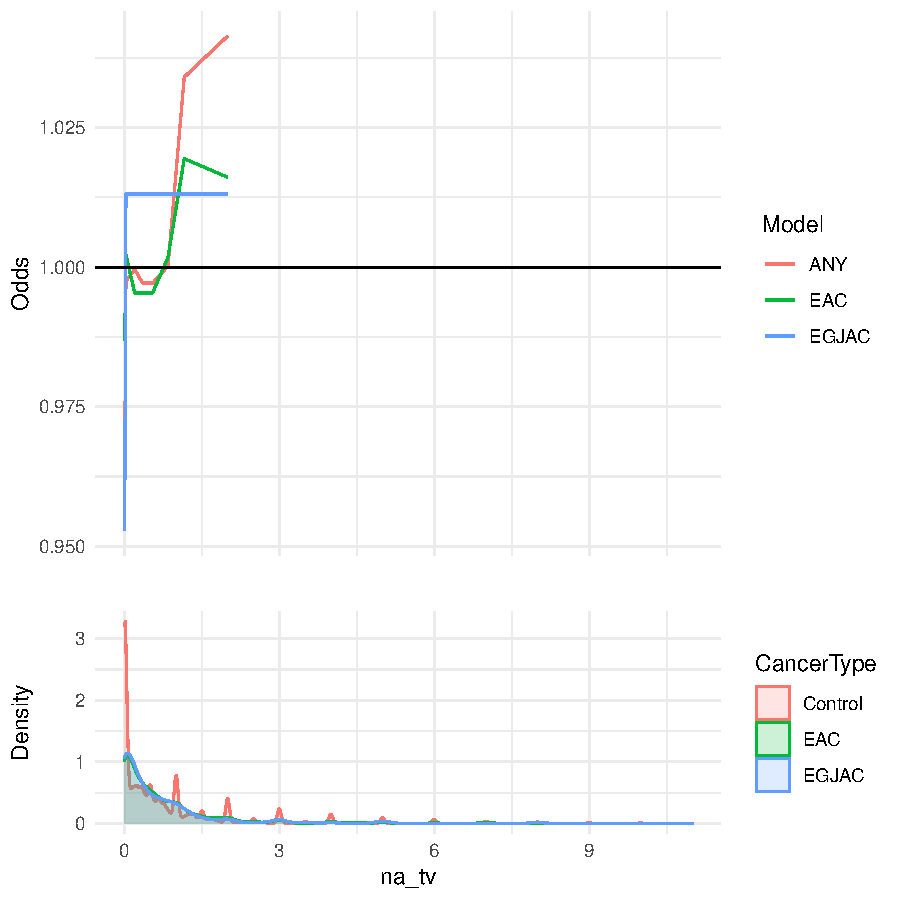
\includegraphics[width=0.45\textwidth]{pdp/na_tv.pdf}
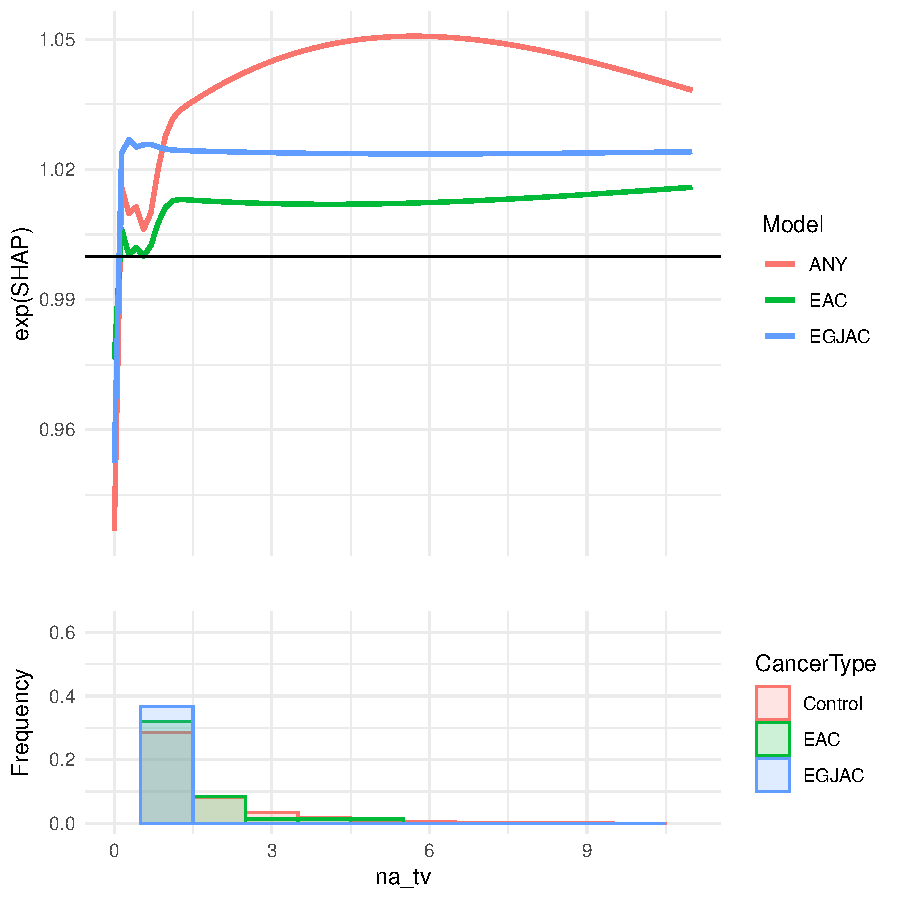
\includegraphics[width=0.45\textwidth]{shap/na_tv.pdf}
\end{figure}




\newpage
\clearpage
\section{BUN}

\begin{figure}[h]
\centering
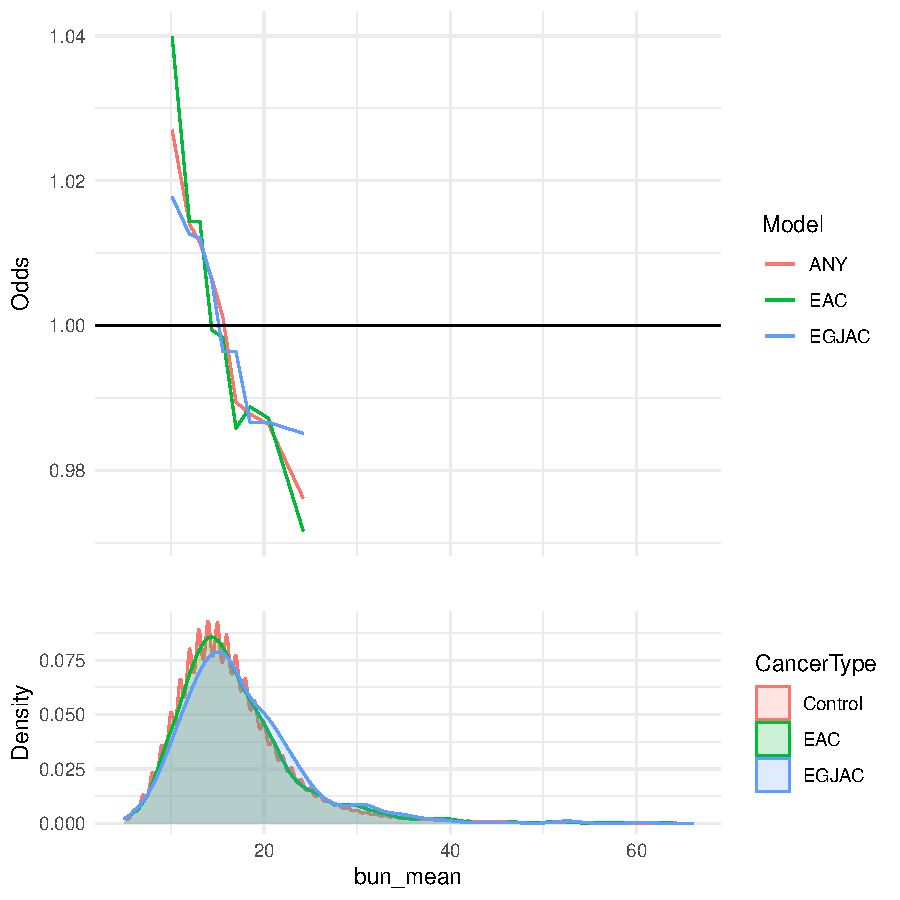
\includegraphics[width=0.45\textwidth]{pdp/bun_mean.pdf}
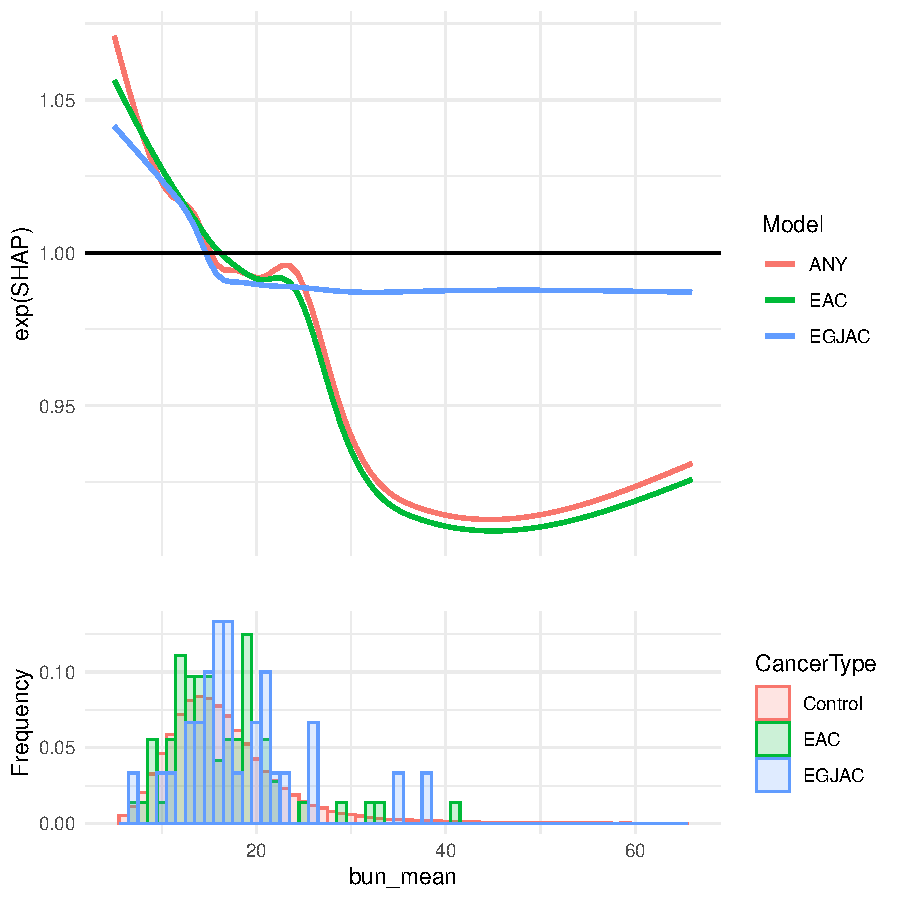
\includegraphics[width=0.45\textwidth]{shap/bun_mean.pdf}
\end{figure}
\begin{figure}[h]
\centering
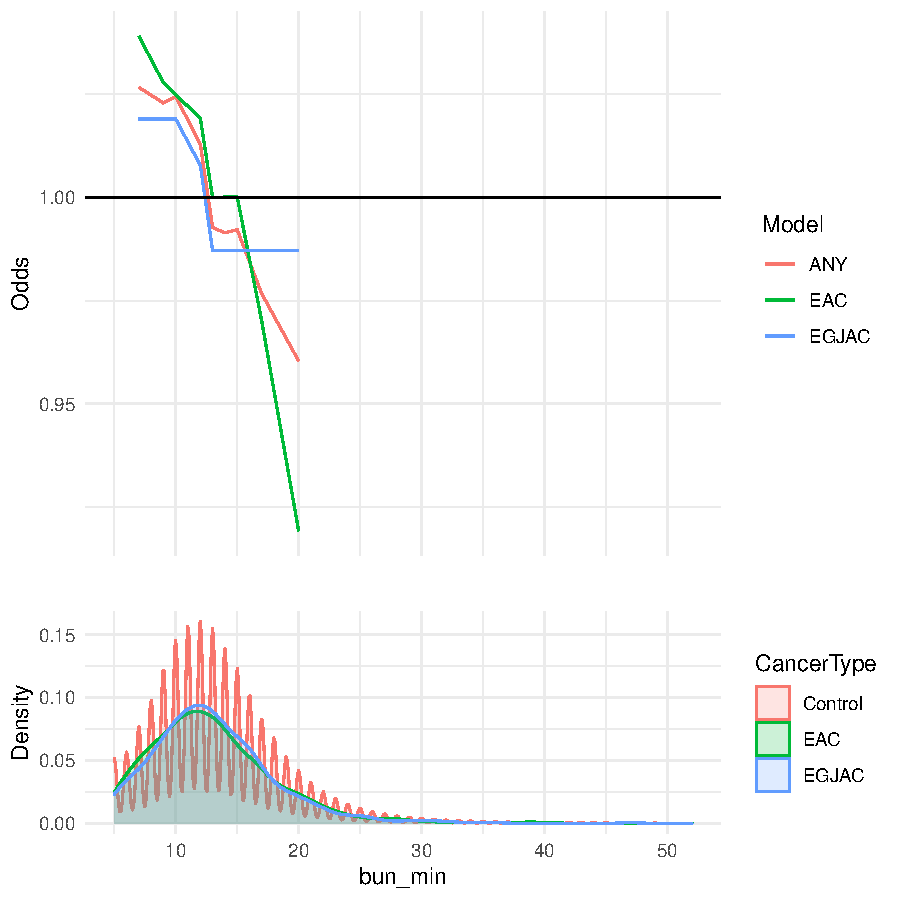
\includegraphics[width=0.45\textwidth]{pdp/bun_min.pdf}
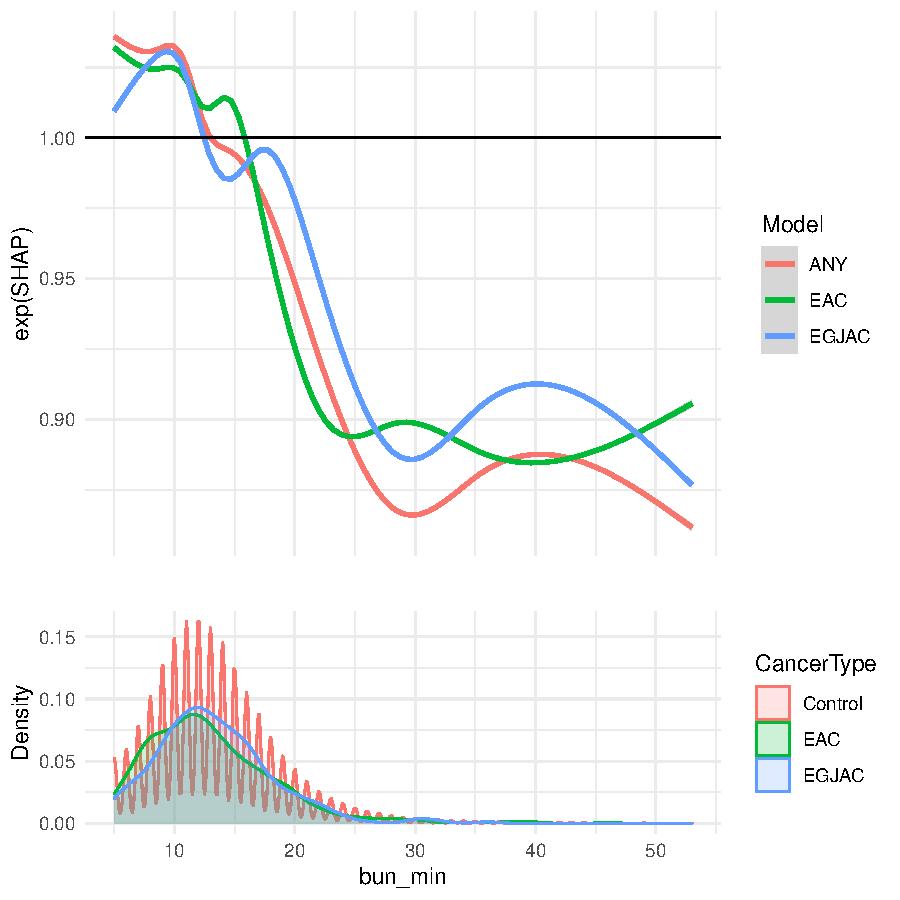
\includegraphics[width=0.45\textwidth]{shap/bun_min.pdf}
\end{figure}
\begin{figure}[h]
\centering
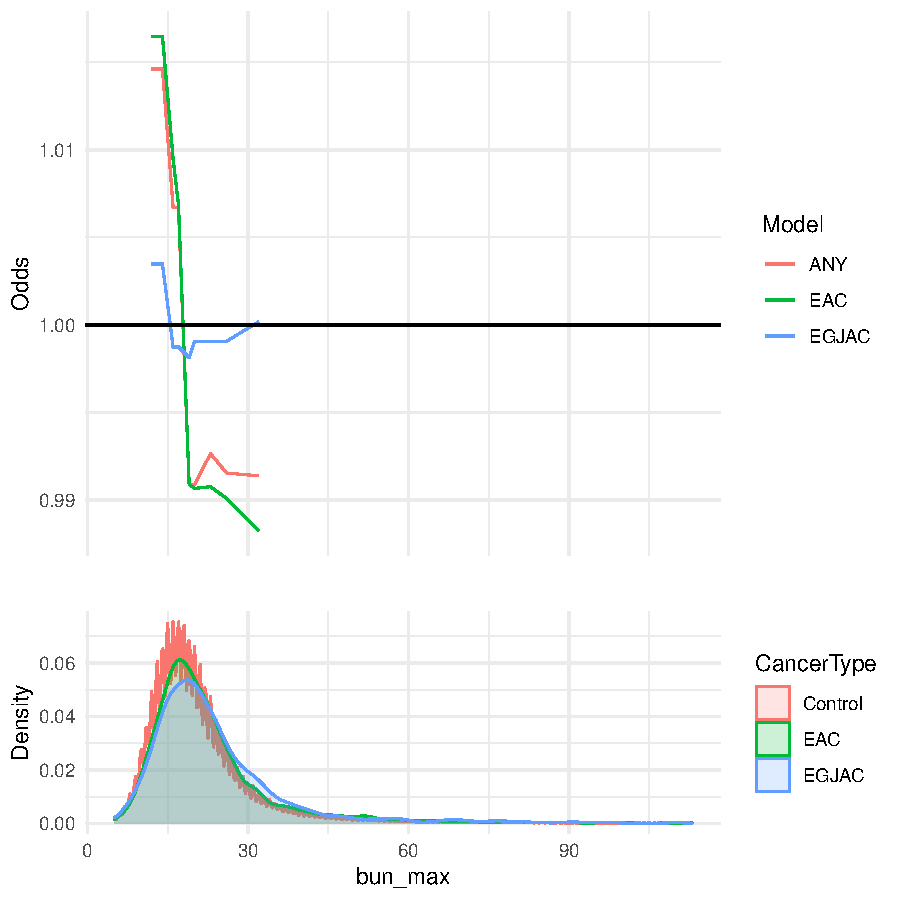
\includegraphics[width=0.45\textwidth]{pdp/bun_max.pdf}
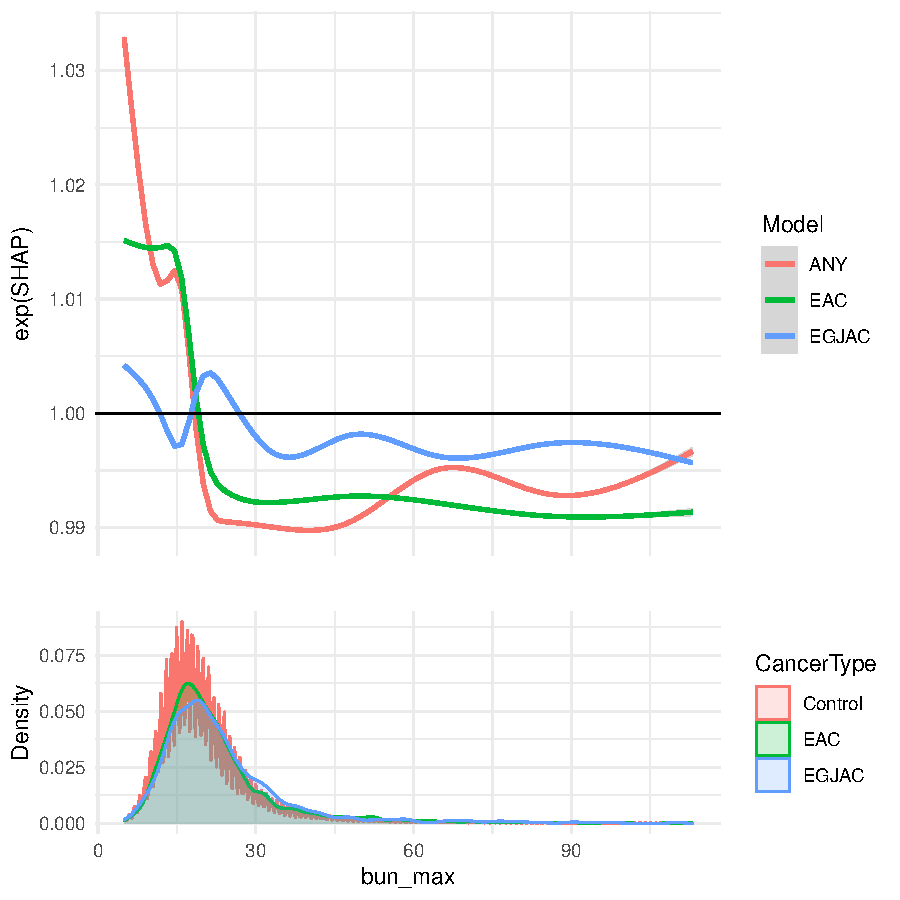
\includegraphics[width=0.45\textwidth]{shap/bun_max.pdf}
\end{figure}
\begin{figure}[h]
\centering
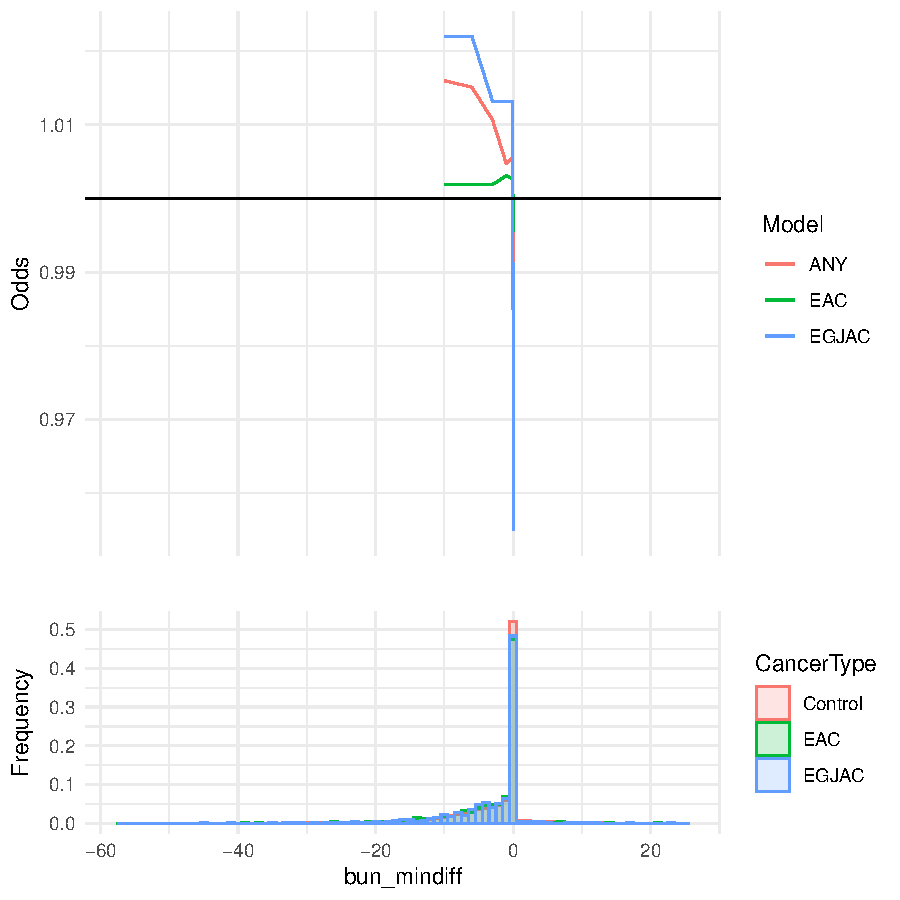
\includegraphics[width=0.45\textwidth]{pdp/bun_mindiff.pdf}
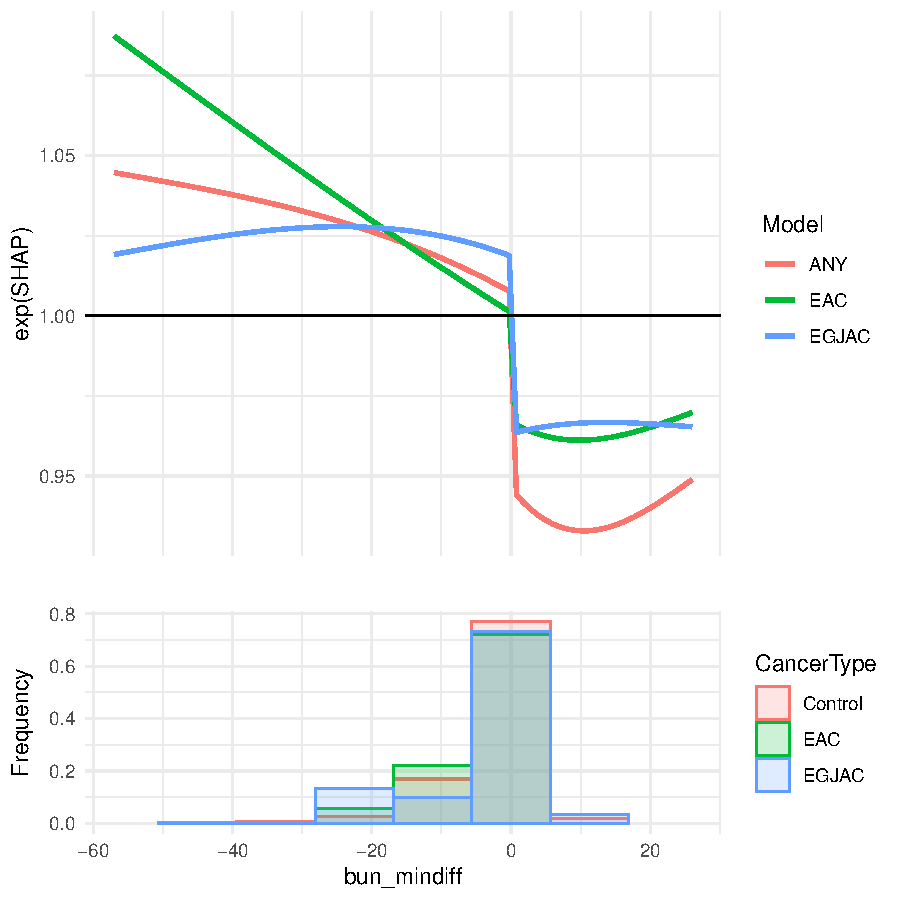
\includegraphics[width=0.45\textwidth]{shap/bun_mindiff.pdf}
\end{figure}
\begin{figure}[h]
\centering
\includegraphics[width=0.45\textwidth]{pdp/bun_maxdiff.pdf}
\includegraphics[width=0.45\textwidth]{shap/bun_maxdiff.pdf}
\end{figure}
\begin{figure}[h]
\centering
\includegraphics[width=0.45\textwidth]{pdp/bun_tv.pdf}
\includegraphics[width=0.45\textwidth]{shap/bun_tv.pdf}
\end{figure}







\end{document}
